\chapter{HeROcache : Applications serverless et coûts associés aux systèmes de stockage}
\label{chapter:herocache}

% TODO: traduction française des figures

\section{Introduction}
\label{section:herocache-introduction}

Dans le chapitre précédent, nous avons vu comment allouer dynamiquement des ressources matérielles et ordonnancer les requêtes utilisateur dans une plateforme serverless pour des applications simples, composées d'une unique fonction, sous contrainte de qualité de service. Un défi important dans le paradigme serverless, lorsque l'on souhaite garantir la qualité de service pour les utilisateurs, survient lors de la composition des fonctions. Ce mécanisme consiste à chaîner des appels de fonctions pour réaliser des tâches complexes, qui induisent des dépendances temporelles et de données. Une chaîne de fonctions est appelée \textit{application} (parfois \textit{workflow}~\cite{burckhardtNetheriteEfficientExecution}). Au cours de l'exécution d'une telle application, les fonctions qui la composent peuvent être instanciées sur tout nœud de l'infrastructure par la plateforme serverless. Leur initialisation provoque des temps de démarrage à froid, et leur dispersion sur les nœuds contribue aux délais de communication qui s'additionnent tout au long de la chaîne, dégradant la qualité de service requise par les différents utilisateurs.

\boitemagique{Question 2 (\textbf{QR2})}{
    Comment déployer des applications complexes, composées de chaînes de fonctions de courte durée, et comment tirer parti de l'hétérogénéité des nœuds disponibles à l'edge, pour respecter la qualité de service requise par les utilisateurs tout en contenant la consommation d'énergie de l'infrastructure ?
    % Comment prendre en compte les délais d'initialisation et de communications lorsque l'on déploie des chaînes de fonctions de courte durée, et comment tirer parti de l'hétérogénéité des nœuds à disposition, pour respecter la qualité de service requise par les utilisateurs et contenir la consommation d'énergie de l'infrastructure ?
}

Le problème que nous abordons dans ce chapitre est celui de la prise en compte par une plateforme serverless des délais d'initialisation et de communication dans des chaînes de fonctions de courte durée de vie, en tirant parti de l'hétérogénéité matérielle pour optimiser le déploiement d'applications sensibles à la latence à l'edge, de manière à garantir une qualité de service variable, tout en limitant le nombre de nœuds edge utilisés. Le travail présenté dans ce chapitre est lié à un projet AID~\footnote{\href{https://www.defense.gouv.fr/aid}{https://www.defense.gouv.fr/aid}} (Agence de l'Innovation de Défense) visant à optimiser le déploiement de systèmes de détection d'intrusion (\textit{IDS}, pour \textit{Intrusion Detection Systems}) sur des plateformes embarquées~\cite{SLIMANI2024}. Ce cas d'étude présente des caractéristiques qui nous intéressent dans le cadre de cette contribution : l'application est critique et clairement définie, composée de plusieurs briques logicielles qui communiquent entre elles ; la plateforme matérielle est hétérogène, et présente des limites en termes de capacité et de performances qui rendent saillants les problèmes soulevés.

Pour déployer des applications sensibles au temps composées de fonctions à courte durée de vie dans un contexte edge, hétérogène et serverless, trois défis doivent être relevés : (1) réduire les délais d'initialisation, (2) éviter des délais de communication élevés et (3) exploiter des ressources hétérogènes pour satisfaire une \gls{QoS} variable :

\begin{enumerate}
    \item \textbf{Délais d'initialisation.} Le serverless s'appuyant sur des ressources non réservées, l'initialisations des fonctions, nécessitant de récupérer leur image depuis un support distant vers les nœuds edge~\cite{yanHermesEfficientCache2020}, peut dégrader la latence des requêtes, surtout dans le cas de fonctions de courte durée comme dans l'IDS -- d'autant plus que les dispositifs edge exposent des supports de stockage de faible capacité et de faible performance, derrière des liaisons réseau limitées en termes de fiabilité et de vitesse.
    \item \textbf{Délais de communication.} Dans une infrastructure distribuée telle que le serverless à l'edge, les fonctions d'une même application peuvent être déployées sur plusieurs nœuds éloignés les uns des autres. Cela implique l'utilisation du réseau, pour exploiter un support de stockage distant lorsque ces fonctions ont besoin de communiquer des résultats intermédiaires. Ces communications par un stockage lent entraînent des retards qui peuvent conduire à des violations de la qualité de service~\cite{wawrzoniakBoxerDataAnalytics2021a}.
    \item \textbf{Hétérogénéité matérielle}. La plateforme serverless ne peut pas considérer tous les placements de tâches comme égaux, car ils produiront différents niveaux de performance : certaines plateformes matérielles sont plus adaptées à certaines tâches. Cependant, l'affinité d'une fonction avec une plateforme d'exécution spécifique ne peut pas guider à elle seule les décisions d'ordonnancement, car ces fonctions peuvent appartenir à différentes chaînes en fonction de l'application demandée. Un placement qui ne prend pas en considération la chaîne de fonctions dans laquelle la requête s'inscrit risque d'entraîner des violations de QoS.
\end{enumerate}

\begin{table*}[!ht]
    \centering
        \caption{État de l'art des plateformes d'orchestration prenant en compte les données}
        \resizebox{\textwidth}{!}{
            \begin{tabular}{lSSSSSSS}
                \toprule
                & Chaînes de fonctions & \gls{QoS} par requête & Hétérogénéité matérielle & Contrainte de programmation & Consommation d'énergie & Cache de fonctions & Communications \\
                \cmidrule(lr){2-2}\cmidrule(lr){3-3}\cmidrule(lr){4-4}\cmidrule(lr){5-5}\cmidrule(lr){6-6}\cmidrule(lr){7-7}\cmidrule(lr){8-8}
                Cypress~\cite{bhasiCypressInputSizesensitive2022} & \cmark & \cmark & \xmark & \cmark & \cmark & \xmark & \cmark \\
                FaDO~\cite{smithFaDOFaaSFunctions2022} & \xmark & \xmark & \xmark & \cmark & \xmark & \xmark & \cmark \\
                FaasFlow~\cite{zijunFassflowEfficient2022} & \cmark & \xmark& \xmark & \xmark & \xmark & \xmark & \xmark \\
                FIRST~\cite{zhangFIRSTExploitingMultiDimensional2023} & \xmark & \xmark & \xmark & \cmark & \cmark & \xmark & \xmark \\
                HeROfake~\cite{herofake} & \xmark & \cmark & \cmark & \cmark & \cmark & \xmark & \xmark \\
                Netherite~\cite{burckhardtNetheriteEfficientExecution} & \cmark & \xmark & \xmark & \cmark & \xmark & \xmark & \cmark \\
                Palette~\cite{abdiPaletteLoadBalancing2023} & \cmark & \xmark & \xmark & \xmark & \xmark & \cmark & \cmark \\
                Target solution & \cmark & \cmark & \cmark & \cmark & \cmark & \cmark & \cmark \\
                \bottomrule
            \end{tabular}
        }
    \label{table:herocache-sota}
\end{table*}

% \textbf{État de l'art.}
Des études antérieures ont exploré le besoin de plateformes d'orchestration qui prennent en charge l'ordonnancement de chaînes de fonctions sur des ressources non réservées. Le tableau~\ref{table:herocache-sota} résume dans quelle mesure ces solutions ne sont pas applicables à notre étude de cas, et la section~\ref{section:herocache-sota} donne plus de détails. Ces contributions visent généralement les déploiements dans le cloud, où l'enjeu est de traiter autant de tâches que possible dans une infrastructure homogène de nœuds toujours en service, afin de maximiser l'usage des ressources. La portée de notre étude est de montrer qu'avec des politiques d'allocation et d'ordonnancement adéquates, nous pouvons déployer des applications bien définies sur un nombre limité de nœuds hétérogènes et réduire la consommation d'énergie globale de l'infrastructure en consolidant les tâches connexes.

% \textbf{Contribution : HeROcache, une plateforme d'orchestration des ressources hétérogènes, optimisée pour la qualité de service, pour le serverless à l'edge et basée sur la mise en cache et la consolidation}.
Dans ce chapitre, nous présentons une solution qui s'appuie sur trois axes pour répondre aux trois défis mentionnés plus haut. HeROcache (1) exploite un mécanisme de mise en cache sur les nœuds edge qui réduit \textbf{les délais d'initialisation} sans saturer leur capacité de stockage ; (2) consolide les tâches sur la base d'une application afin de limiter la durée des \textbf{délais de communication} entre les fonctions ; (3) gère le respect des exigences de qualité de service pour les tâches critiques en utilisant des métadonnées collectées auprès des applications et des plateformes hétérogènes utilisées pour le déploiement. Ces données comprennent des mesures de performance et d'énergie qui guident l'orchestrateur dans ses prises de décision, lors de l'allocation de ressources et de l'ordonnancement de requêtes toutes \textbf{hétérogènes}.

% \textbf{Quelques résultats.}
Nous avons évalué HeROcache dans le contexte d'une application d'IDS réelle, caractérisée sur différentes plateformes d'exécution. Cette évaluation a été réalisée à l'aide d'un simulateur, présenté au chapitre~\ref{chapter:herosim}, dans lequel nous avons également mis en œuvre le comportement d'un orchestrateur Knative~\cite{knative}. HeROcache parvient à surpasser Knative, en maintenant les violations de la qualité de service à moins de 28\% tout en consolidant les tâches sur 20\% des nœuds edge de l'infrastructure. La mise hors tension de ces nœuds entraînerait une réduction drastique de la consommation d'énergie statique.

Le chapitre est organisé comme suit : la section~\ref{section:herocache-background} détaille les défis pour le déploiement de l'IDS sur une plateforme serverless ; la section~\ref{section:herocache-before-contrib} présente le projet et son architecture globale ; la section~\ref{section:herocache-workload} détaille notre approche de collecte de métadonnées hors-ligne ; la section~\ref{section:herocache-contribution} décrit notre stratégie d'orchestration en ligne ; la section~\ref{section:herocache-evaluation} discute des résultats de l'évaluation ; la section~\ref{section:herocache-sota} discute de travaux connexes de l'état de l'art ; enfin, la section~\ref{section:herocache-conclusion} conclut le chapitre en donnant des limites à cette contribution et des perspectives pour de futurs travaux.

\section{Contexte et motivation}
\label{section:herocache-background}

\subsection{Détection d'intrusion à l'edge}

% \textbf{Les IDS, des applications critiques et sensibles au temps.}
Un large éventail de systèmes embarqués fonctionnant dans des environnements statiques et contrôlés (capteurs dans une usine) ou dynamiques et non contrôlés (essaims de drones en mouvement) peuvent être temporairement ou constamment exposés à des attaques critiques par l'intermédiaire de liaisons réseau. Comme ces attaques peuvent compromettre leur exécution et endommager gravement les infrastructures connexes, il est essentiel de les prendre en compte. Pour atténuer ces menaces, les systèmes de détection d'intrusion sont utilisés pour analyser le trafic réseau et détecter des motifs d'activités potentiellement malveillantes. Les modèles d'apprentissage machine sont particulièrement utiles pour classifier ce trafic, mais ils sont très gourmands en ressources de calcul, en mémoire et en stockage. Par conséquent, les exécuter directement sur la plateforme embarquée n'est pas une solution sûre, car cela peut affecter leur durée de vie s'ils fonctionnent sur une batterie~\cite{slimani:hal-04159551}, interférer avec d'autres tâches critiques, ou même être totalement impossible en raison d'un manque de ressources.

% \textbf{IDS à l'edge.}
Pour décharger les systèmes embarqués de l'exécution de ces algorithmes gourmands en ressources, tout en maintenant le système réactif aux attaques, une solution consiste à exécuter les \gls{IDS} dans le cloud, et en particulier sur les dispositifs \textit{edge}~\cite{eskandari2020}. Les IDS doivent répondre à des exigences variables en matière de qualité de service (\gls{QoS}) et peuvent n'être nécessaires que pendant des périodes critiques, identifiées à l'avance. En outre, différents types d'attaques peuvent présenter des risques différents sur l'infrastructure sous-jacente, et le risque d'attaque peut varier dans le temps et dans l'espace (en fonction du domaine d'application). Par conséquent, il pourrait être inutilement coûteux de déployer des systèmes de détection d'intrusion sur des dispositifs edge réservés. Nous soutenons que le déploiement d'IDS sur des ressources non réservées à faible consommation d'énergie à l'edge pourrait offrir l'avantage d'une solution rentable pour l'exécution de telles applications, tout en offrant une latence plus faible que lorsque l'on s'appuie sur le cloud.

% \subsection{Défis de l'orchestration dynamique}
\subsection{Défis de l'orchestration dynamique d'applications critiques à l'edge}

% \textbf{Serverless et IDS à l'edge.}
L'un des principaux paradigmes du cloud qui permet d'exécuter des applications interactives sur des ressources non réservées, avec une granularité fine d'allocation des ressources, est le serverless~\cite{Lannurien2023}. Le déploiement serverless à l'edge pour l'\gls{IDS}, et plus généralement pour les applications critiques et sensibles au temps, peut être intéressant du point de vue des coûts en ouvrant des possibilités d'optimisation pour le fournisseur de services, grâce à la mise à l'échelle dynamique des ressources suite à des pics de charge dans les applications interactives, ainsi qu'à une granularité d'allocation fine et mesurée pour les ressources limitées à l'edge.

% \textbf{Défis pour le déploiement serverless d'applications critiques à l'edge.}
% Pour déployer des applications sensibles au temps composées de fonctions à courte durée de vie dans un contexte edge, hétérogène et serverless, trois défis doivent être relevés : (1) réduire les délais d'initialisation, (2) éviter des délais de communication élevés et (3) exploiter des ressources hétérogènes pour satisfaire une \gls{QoS} variable.
% \textbf{Délais d'initialisation.} Le serverless s'appuyant sur des ressources non réservées, le taux d'initialisations de fonctions, nécessitant de récupérer l'image de la fonction depuis un support distant vers les nœuds edge~\cite{yanHermesEfficientCache2020}, peut dégrader la latence des requêtes, surtout dans le cas de fonctions de courte durée comme dans l'IDS -- d'autant plus que les dispositifs edge exposent des supports de stockage de faible capacité et de faible performance, derrière des liaisons réseau limitées en termes de fiabilité et de vitesse. Cette première problématique doit donc être adressée pour satisfaire la qualité de service des utilisateurs.
% \textbf{Délais de communication.} Dans une infrastructure distribuée telle que le serverless à l'edge, les fonctions d'une même application peuvent être déployées sur plusieurs nœuds éloignés les uns des autres. Cela implique l'utilisation du réseau, pour exploiter un support de stockage distant lorsque ces fonctions ont besoin de communiquer des résultats intermédiaires. Ces communications par un stockage lent entraînent des retards qui peuvent conduire à des violations de la qualité de service~\cite{wawrzoniakBoxerDataAnalytics2021a}.
% \textbf{Hétérogénéité matérielle}. La plateforme serverless ne peut pas considérer tous les placements de tâches comme égaux, car ils produiront différents niveaux de performance : certaines plateformes matérielles sont plus adaptées à certaines tâches. Cependant, l'affinité d'une fonction avec une plateforme d'exécution spécifique ne peut pas guider à elle seule les décisions d'ordonnancement, car ces fonctions peuvent appartenir à différentes chaînes en fonction de l'application demandée. Un placement qui ne prend pas en considération la chaîne de fonctions dans laquelle la requête s'inscrit risque d'entraîner des violations de QoS.

% Le serverless est un modèle de service en croissance pour le cloud~\cite{Lannurien2023} : en transférant la responsabilité de l'allocation des ressources des clients vers les fournisseurs de services, il allège une partie importante de la complexité pour les développeurs d'applications et ouvre de nouvelles possibilités d'optimisation et de contrôle des coûts pour le gestionnaire d'infrastructure. Dans une architecture serverless, les développeurs conçoivent leurs applications comme une composition de fonctions sans état. Sans état (ou "pur", sans effet secondaire) signifie que le résultat du calcul dépend exclusivement des entrées \cite{burckhardtNetheriteEfficientExecution}. Ces fonctions prennent en entrée une charge utile et un contexte d'invocation, et produisent un résultat qui est stocké dans un niveau de stockage persistant accessible par le réseau. Cela signifie que les dépendances de données entre les fonctions d'une chaîne doivent être gérées par la plateforme.

Lorsqu'un événement déclenche leur exécution, les fonctions sont déployées sur des nœuds de l'infrastructure, dans des environnements d'exécution appelés \textbf{répliques}. Comme les fonctions sont sans état, les requêtes peuvent être attribuées à n'importe quelle réplique disponible. La mise à l'échelle d'une application serverless, \textit{i.e.} pour maintenir un niveau de performance constant, consiste à faire croître ou décroître le nombre de répliques des fonctions en suivant les pics de charge. Les plateformes serverless basées sur Kubernetes, telles que Knative~\cite{knative} ou OpenWhisk~\cite{openwhisk}, ont proposé un modèle basé sur un seuil de concurrence pour le dimensionnement du pool de répliques. Pour toute fonction, un \textbf{autoscaler} peut déployer plusieurs \textit{répliques} pour absorber la charge. Chaque réplique est allouée à une plateforme d'exécution (\textit{i.e.} un cœur de CPU, un GPU, etc.) et dispose d'une file d'attente pour les requêtes entrantes. Le nombre de répliques pour une fonction donnée à un instant donné détermine son niveau de concurrence. Un \textbf{ordonnanceur} place les requêtes utilisateur dans la file d'attente d'une réplique de la fonction. Lorsqu'une réplique n'a plus de requêtes en attente, elle peut être détruite. Lorsqu'une fonction est demandée alors qu'aucune réplique n'existe, elle passe par un \textbf{démarrage à froid} qui entraîne un délai d'initialisation qui s'ajoute au temps de réponse de la fonction.

% Dans le serverless, la fréquence des allocations de ressources augmente considérablement par rapport aux environnements à ressources réservées, toujours actives, tels que les offres IaaS ou PaaS (cf. chapitre~\ref{chapter:context}). La capacité des plateformes serverless à mettre à l'échelle une fonction jusqu'à zéro réplique afin d'éviter de facturer les clients pour des ressources inactives est une différence essentielle par rapport aux modèles de services cloud traditionnels.

Ce démarrage à froid présente un risque d'augmentation du temps de réponse d'une application, car la plateforme doit allouer des ressources matérielles pour instancier chacune des fonctions qui la composent avant de répondre à la requête. Plus l'application est complexe, plus le risque de retards cumulés est élevé~\cite{mohanAgileColdStartsa}. Les fournisseurs pré-allouent généralement certaines ressources pour éviter les démarrages à froid, ce qui a un coût en termes de provisionnement des ressources. Les acteurs commerciaux tels qu'AWS, Google et Microsoft réutilisent tous, dans une certaine mesure, des instances de fonctions, en les gardant en vie pendant une période de grâce afin d'éviter les coûts en latence induits par les démarrages à froid~\cite{vahidiniaColdStartServerless2020}.

Une étude récente a montré que 50\% des applications serverless déployées sur Microsoft Azure Durable Functions~\footnote{\href{https://learn.microsoft.com/en-US/azure/azure-functions/durable/durable-functions-overview}{https://learn.microsoft.com/en-US/azure/azure-functions/durable/durable-functions-overview}} sont constituées de 3 fonctions ou moins, 65\% des applications présentant un simple DAG (\textit{Directed Acyclic Graph}, graphe acyclique dirigé) de fonctions agencées sous forme de chaînes linéaires \cite{mahgoubORIONThreeRights}. Notre application d'IDS se compose de différentes chaînes de deux fonctions, comme décrit dans la section~\ref{section:herocache-characterization-workloads}. Des travaux de caractérisation des charges de travail serverless ont montré que 25\% des fonctions déployées sur Microsoft Azure Functions~\footnote{\href{https://azure.microsoft.com/en-us/products/functions/}{https://azure.microsoft.com/en-us/products/functions/}} s'exécutent en 100 ms ou moins \cite{shahradServerlessWildCharacterizing}. Les fonctions qui composent notre application d'IDS s'exécutent pendant quelques centièmes ou dixièmes de seconde, ce qui les rend particulièrement sujettes à des ralentissements critiques dans le contexte de l'allocation dynamique des ressources.

\subsection{Mise en cache des images de fonctions}
\label{section:herocache-background-cache}

\begin{figure}[!ht]
    \centering
    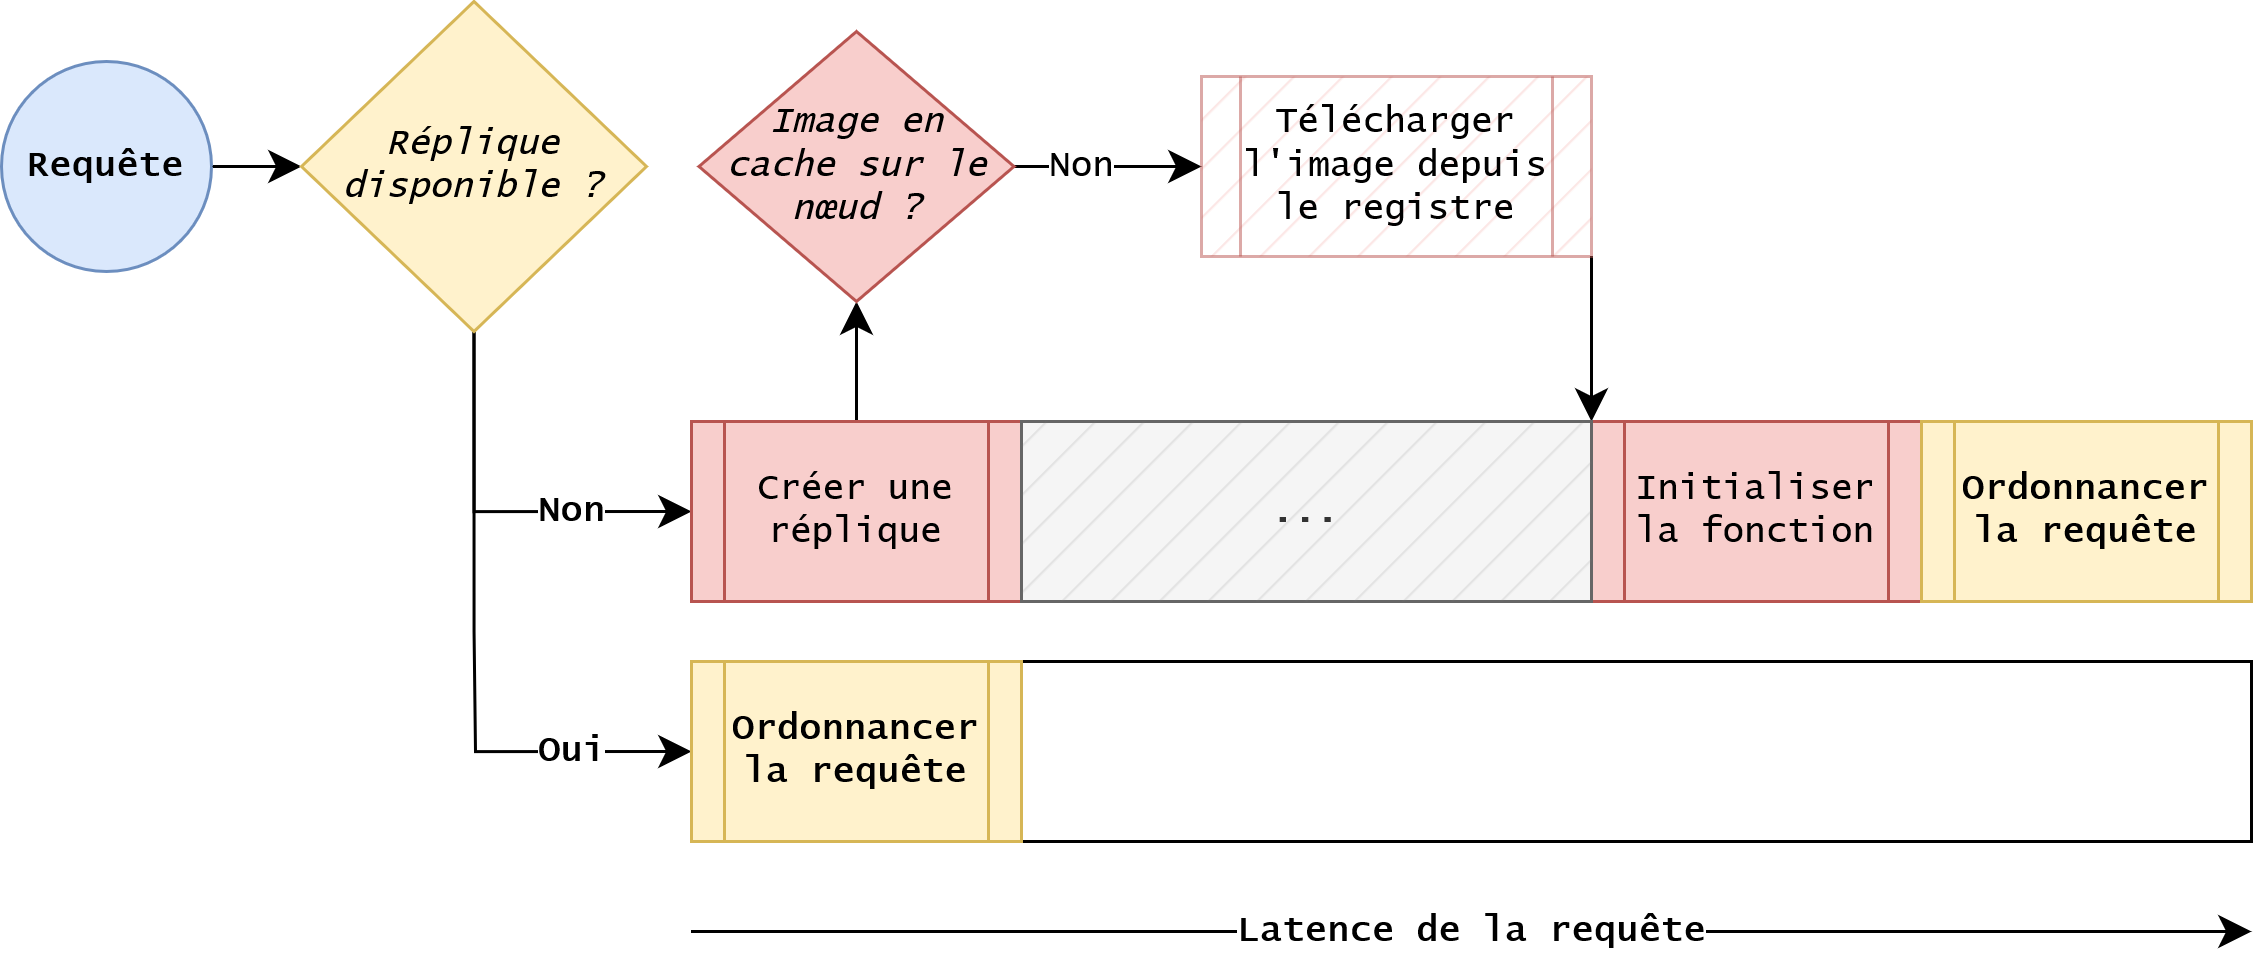
\includegraphics[width=0.8\columnwidth]{5_Chapitre5/figures/function-cache.png}
    \caption{Cycle de vie d'une requête utilisateur dans une plateforme serverless. L'arrivée d'une requête dans le système provoque des décisions de mise à l'échelle (en rouge) et d'ordonnancement (en jaune).}
    \label{figure:herocache-function-cache}
\end{figure}

Afin de répondre aux requêtes des utilisateurs sans dégrader les performances, l'autoscaler ajuste périodiquement le nombre de répliques pour chaque fonction déployée : le pool de répliques croît et décroît en fonction des variations sur la charge des fonctions d'une application. Lorsque la charge sur une fonction augmente au-delà du seuil de concurrence de la plateforme, l'autoscaler crée une nouvelle réplique qui traitera les requêtes supplémentaires des utilisateurs. Lorsque la charge diminue, les répliques inactives sont supprimées. S'il n'y a plus de requêtes pour une fonction donnée, celle-ci peut être \textit{mise à l'échelle jusqu'à zéro}, ce qui permet de réattribuer des ressources matérielles à des tâches plus pressantes.

Les répliques de fonctions sont initialisées à partir d'\textbf{images de fonctions} (\textit{e.g.} une image Docker ou de machine virtuelle). Celles-ci sont stockées dans un registre d'images. Ces registres peuvent être accessibles à distance par Internet, ou déployés dans l'infrastructure du fournisseur. Toutefois, de nombreuses études antérieures~\cite{bhasiCypressInputSizesensitive2022, zijunFassflowEfficient2022, smithFaDOFaaSFunctions2022, zhangFIRSTExploitingMultiDimensional2023} n'envisagent que des scénarios favorables, dans lesquels les images de fonctions sont déjà disponibles sur les nœuds edge. Cela ne reflète pas la réalité, puisque les images de fonctions sont stockées dans des registres, sur des nœuds dédiés, et téléchargées sur les nœuds edge lors du déploiement des fonctions (figure~\ref{figure:herocache-function-cache}). En fonction de la taille de l'image, cela peut avoir des conséquences négatives sur la latence des requêtes avec des déploiements où les démarrages à froid dominent le temps de réponse total d'une fonction \cite{yanHermesEfficientCache2020}.

Ce processus d'initialisation des répliques à partir d'images sur les nœuds edge peut représenter jusqu'à 80\% du temps de réponse d'une fonction \cite{yanHermesEfficientCache2020} dans les cas où la latence introduite par le démarrage à froid domine le temps de réponse total de la fonction. Cette situation n'est pas acceptable lorsque la plateforme doit répondre à des exigences strictes en matière de qualité de service, comme c'est le cas pour les tâches critiques telles que l'IDS.

\subsection{Communications entre les fonctions}
\label{section:herocache-background-communications}

\begin{figure}[!ht]
    \centering
    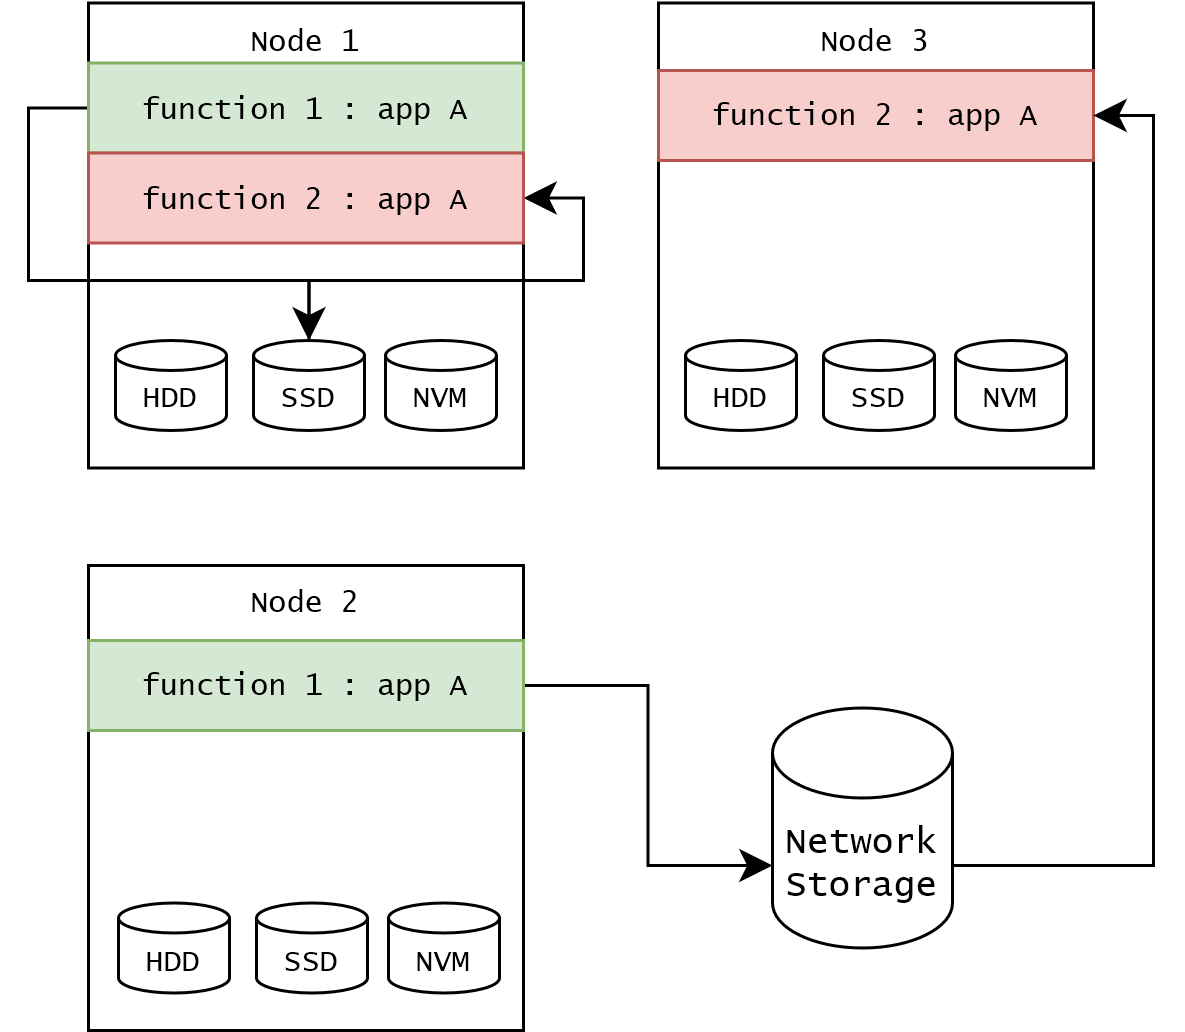
\includegraphics[width=0.8\columnwidth]{5_Chapitre5/figures/function-communications.png}
    \caption{Les fonctions serverless communiquent des résultats intermédiaires à travers un stockage persistant, qui peut être local aux nœuds et rapide (cas du premier nœud de la figure), ou accédé par le réseau et lent (cas des nœuds 2 et 3).}
    \label{figure:herocache-function-communications}
\end{figure}

Pour rendre possible la mise à l'échelle dynamique des fonctions, il est nécessaire que chaque invocation d'une fonction serverless soit indépendante, c'est-à-dire qu'elle ne porte pas les données ou le contexte des invocations précédentes. Cela permet aux répliques de mettre en file d'attente les requêtes utilisateur et de les traiter de manière séquentielle sans avoir besoin de procéder à un démarrage à froid entre les requêtes. Cela introduit une contrainte sur la plateforme serverless : si une application est composée de plusieurs fonctions qui forment une chaîne de traitement, la sortie de chaque fonction doit être sauvegardée dans un stockage persistant pour être passée en entrée de la fonction suivante dans la chaîne~\cite{mullerLambadaInteractiveData2020} (figure~\ref{figure:herocache-function-communications}).

Les travaux de l'état de l'art ont montré que les fonctions serverless qui communiquent, \textit{via} le réseau, par le biais d'un stockage distant, peuvent subir un ralentissement jusqu'à 11x par rapport aux fonctions utilisant des communications directes~\cite{wawrzoniakBoxerDataAnalytics2021a} (\textit{e.g.} au travers de mémoire partagée au sein d'un même nœud). Les fonctions de notre application d'IDS doivent communiquer des résultats intermédiaires à chaque étape du DAG de l'application. Lorsque les fonctions sont déployées sur différents nœuds edge, les communications inter-fonctions devront être réalisées par l'utilisation d'un stockage à distance. Cela introduit des ralentissements qui peuvent faire boule de neige tout au long de l'exécution des fonctions et détériorer la qualité de service de l'ensemble de l'application.

\section{Détection d'intrusion à l'edge dans le modèle serverless}
\label{section:herocache-before-contrib}

\begin{figure*}[!ht]
    \centering
    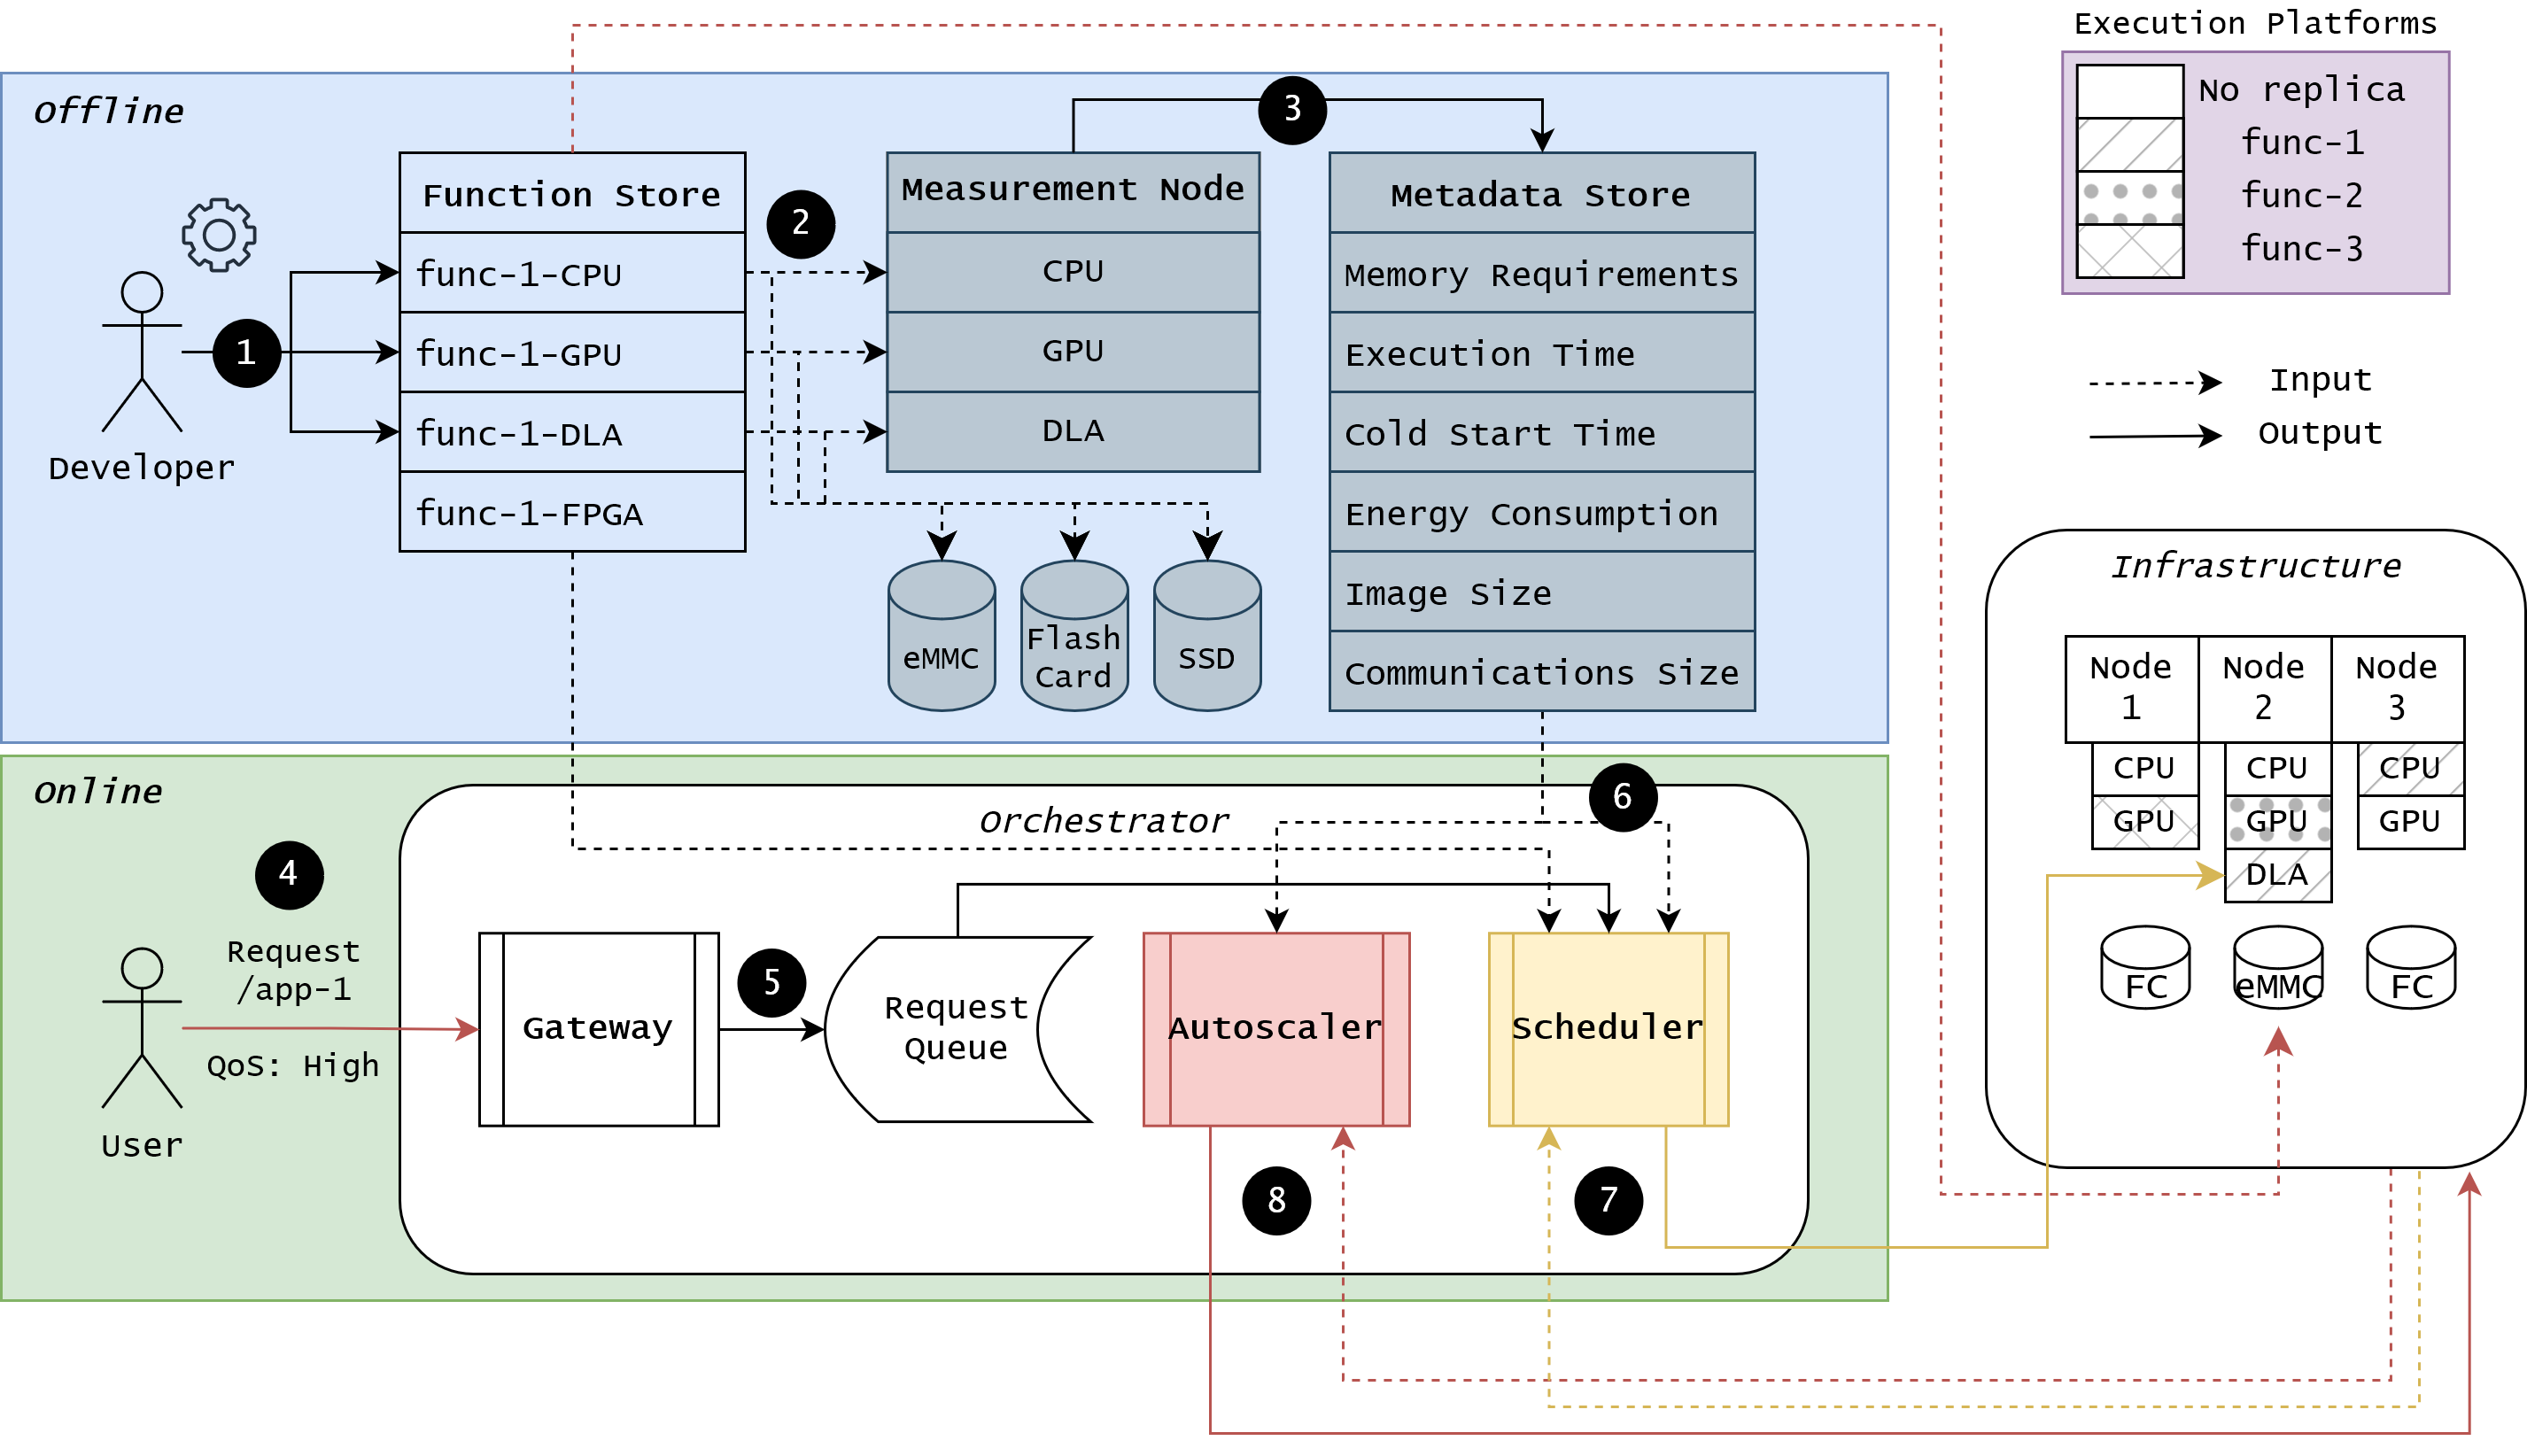
\includegraphics[width=0.75\textwidth]{5_Chapitre5/figures/serverless-platform-storage.png}
    \caption{Plateforme serverless pour le déploiement d'une application d'\gls{IDS}.}
    \label{figure:herocache-serverless-platform}
\end{figure*}

Orchestrer des applications tout en respectant les accords de niveau de service (\gls{SLA}, pour \textit{Service Level Agreement}) nécessite de modéliser précisément les caractéristiques de l'application et d'en tenir compte lors de l'allocation des ressources et de l'ordonnancement des requêtes utilisateur sur la plateforme serverless. La figure~\ref{figure:herocache-serverless-platform} donne un aperçu du cycle de vie d'une application sur notre plateforme. Il est divisé en deux phases ; une \textbf{phase hors-ligne} qui consiste à caractériser les applications déployées par les développeurs sur les plateformes edge, et une \textbf{phase en ligne} où les requêtes des utilisateurs vers ces applications sont ordonnancées sur la plateforme.

\textbf{Phase hors-ligne}. Dans notre plateforme, le cycle de vie de l'application commence par une phase hors-ligne, au cours de laquelle le développeur fournit le code de ses fonctions pour différentes architectures matérielles (\gls{GPU}, \gls{CPU}, \gls{DLA}, etc.)~\Circled{1}. Ce code est stocké par le fournisseur de services dans un registre de fonctions. Les fonctions sont ensuite déployées sur un nœud de mesure~\Circled{2} où elles sont exécutées afin de produire des métadonnées relatives à leur exécution sur des nœuds hétérogènes. Les besoins en mémoire, le temps d'exécution, le temps de démarrage à froid, la consommation d'énergie, la taille de la fonction et la taille des données communiquées pour chaque fonction sont enregistrés dans un registre de métadonnées~\Circled{3}. L'exécution de la phase hors-ligne est nécessaire une fois pour une fonction donnée sur une plateforme donnée, comme décrit dans la section~\ref{section:herocache-workload}.

\textbf{Phase en ligne}. Les requêtes utilisateur envoyées aux applications d'\gls{IDS} comportent un extrait de trafic réseau (sous forme de paquets \gls{TCP}, pour \textit{Transmission Control Protocol}, sérialisés) à analyser~\Circled{4}, et sont associées à un niveau de qualité de service souhaité pour le temps de réponse de la requête. La requête est ajoutée à une file d'attente~\Circled{5} au niveau de l'orchestrateur. Lorsque l'ordonnanceur extrait la requête de la file d'attente, il interroge le registre pour récupérer les métadonnées de fonction appropriées~\Circled{6}.

L'ordonnanceur tente alors de trouver une réplique disponible de la première fonction de l'application pour traiter la requête~\Circled{7}. Si une telle réplique n'existe pas encore, il sera demandé à l'autoscaler d'initialiser une nouvelle instance de la fonction~\Circled{8}. Au cours du cycle de vie de l'application, l'autoscaler vérifie périodiquement la charge moyenne de chaque fonction pour ajuster le nombre de répliques déployées sur la plateforme, en fonction du seuil de concurrence fixé par le fournisseur de services.

Lorsque l'application termine son exécution, elle retourne à l'utilisateur un vecteur de classification qui indique les probabilités que le trafic soit malveillant, c'est-à-dire qu'il présente les caractéristiques d'une attaque potentielle.

\section{Phase hors-ligne : caractérisation} 
\label{section:herocache-workload}

\begin{figure}[!ht]
    \centering
    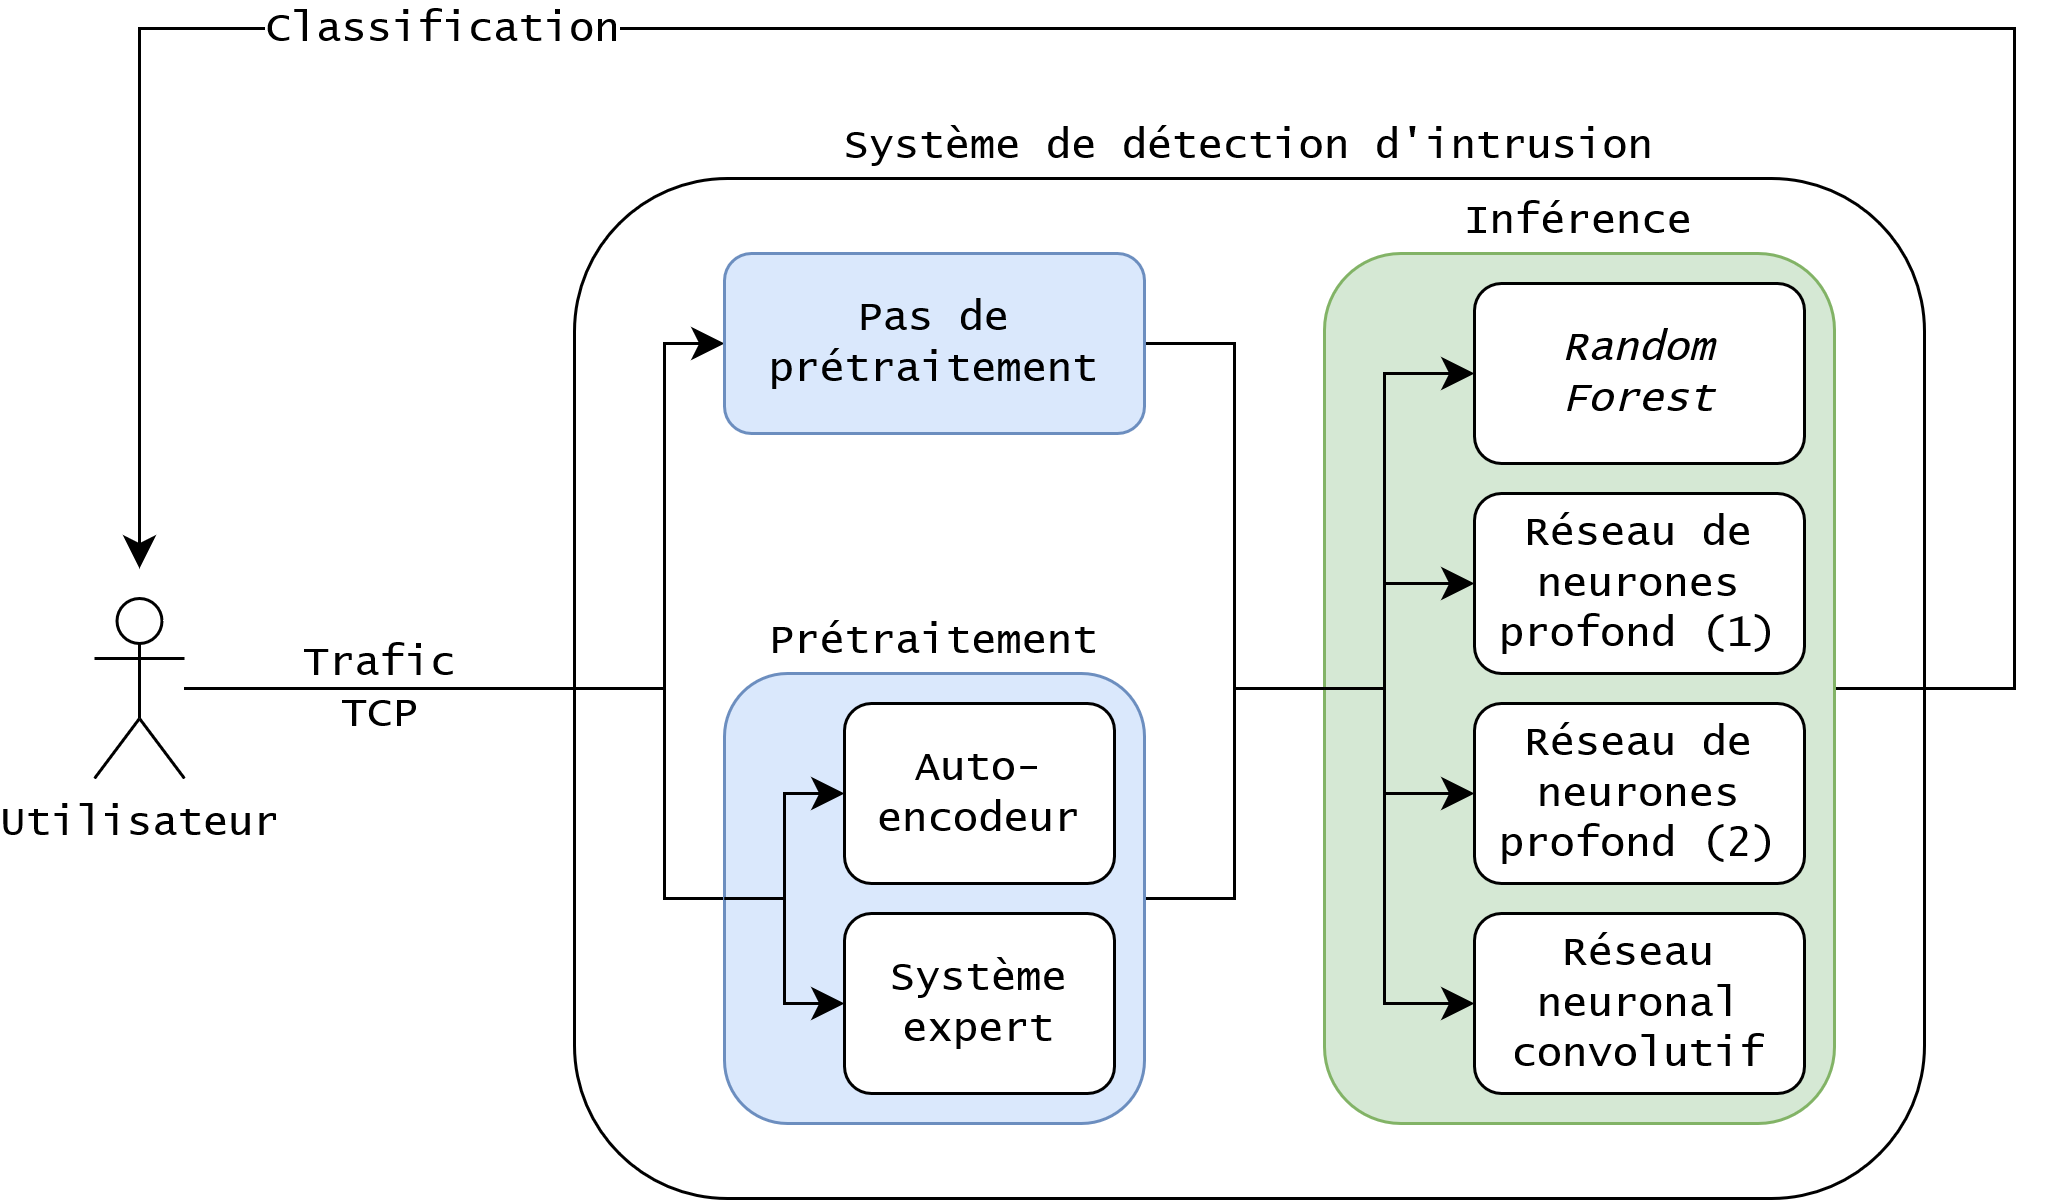
\includegraphics[width=0.8\columnwidth]{5_Chapitre5/figures/ids-application.png}
    \caption{Architecture de l'application d'IDS. Elle peut exploiter différentes fonctions de prétraitement, et différentes fonctions d'inférence pour fournir une classification du trafic \gls{TCP} à l'utilisateur.}
    \label{figure:herocache-ids-application}
\end{figure}

Pour parvenir à une allocation des ressources et à un placement des tâches adéquats lors de l'exécution des applications d'\gls{IDS}, il est nécessaire de caractériser les plateformes d'exécution ainsi que les fonctions logicielles qui seront mobilisées~\cite{mampageHolisticViewResource2022}. À cette fin, nous avons évalué plusieurs modèles de détection d'intrusion en termes de performance et de consommation d'énergie sur des plateformes hétérogènes représentatives de dispositifs edge~\cite{kljucaric2020}. Cette section décrit notre méthodologie et nos résultats.

\subsection{Caractérisation des plateformes d'exécution} \label{section:herocache-characterization-platforms}

Nous avons utilisé des plateformes représentatives de ce que l'on peut trouver à l'edge~\cite{slimani:hal-04159551,kljucaric2020} :
\textbf{(1) Raspberry Pi 4B}, équipée d'un CPU quadricœur ARM Cortex-A72, de 4 GB LPDDR4 en mémoire principale et d'une carte SD de 16 GB. La carte fonctionne sous Linux 5.4, avec la distribution Raspbian.
\textbf{(2) Nvidia Jetson Xavier AGX}, composée de trois éléments de traitement : un CPU NVIDIA ARM Carmel à 8 cœurs, un GPU NVIDIA Volta avec 512 cœurs CUDA et un accélérateur d'apprentissage profond (\textit{DLA}, pour \textit{Deep Learning Accelerator}), qui est un accélérateur matériel à fonction fixe conçu pour les réseaux neuronaux convolutifs (\textit{CNN}, pour \textit{Convolutional Neural Network}). Il est supposé être plus économe en énergie que le GPU. La carte Xavier AGX est équipée de 16 GB de mémoire LPDDR4 et de 32 GB de mémoire flash eMMC 5.1. Elle fonctionne sous Linux Tegra 4.9.10. Le mode d'alimentation \textit{15 Watts Desktop} a été utilisé.
\textbf{(3) PYNQ-Z2 Development Board}, une carte basée sur le système sur puce (\textit{SoC}, pour \textit{System on Chip}) Xilinx Zynq XC7Z020. Elle est équipée d'un FPGA Artix-7, d'une mémoire DDR3 de 512 MB et d'une carte SD de 16 GB.

\subsection{Caractérisation des applications}
\label{section:herocache-characterization-workloads}

Notre application, schématisée en figure~\ref{figure:herocache-ids-application}, se compose de différents préprocesseurs et classificateurs. Le préprocesseur sélectionne un sous-ensemble de caractéristiques pertinentes des paquets \gls{TCP} fournis par l'utilisateur. Trois approches de prétraitement différentes ont été retenues : (1) utilisation de toutes les caractéristiques des paquets sans aucune sélection (\textit{NoFS}, pour \textit{No Feature Selection}) ; (2) utilisation d'un auto-encodeur \textit{DNN} (\textit{Deep Neural Network}) pour projeter les caractéristiques dans un espace latent plus petit (\textit{AE}, pour \textit{Auto-Encoder}) ; et (3) sélection experte d'un sous-ensemble de caractéristiques (\textit{ES}, pour \textit{Expert Selection}). Pour la partie classification, nous avons utilisé un algorithme de \textit{Random Forest} (\textit{RF}), deux architectures différentes de réseaux neuronaux denses (\textit{DNN}) et un \textit{CNN}.

\begin{table}[t]
\caption{IDS models architecture and size}
\resizebox{\textwidth}{!}{
\begin{tabular}{|c|c|cc|}
\hline
Model     & Architecture                                                                                                                                         & \multicolumn{1}{c|}{Model Size on CPUs (MB)} & Model Size on GPU (MB) \\ \hline
NoFS-RF   & \begin{tabular}[c]{@{}c@{}}5 trees of 100\\ maximum depth\end{tabular}                                                                               & \multicolumn{1}{c|}{28}                      & 15.4                   \\ \hline
AE-RF     & \begin{tabular}[c]{@{}c@{}}5 trees of 50 \\ maximum depth\end{tabular}                                                                               & \multicolumn{1}{c|}{-}                       & 32.9                   \\ \hline
ES-RF     & \begin{tabular}[c]{@{}c@{}}10 trees of 10 \\ maximum depth\end{tabular}                                                                              & \multicolumn{1}{c|}{9.1}                     & 5.5                    \\ \hline
NoFS-DNN1 & \multirow{3}{*}{\begin{tabular}[c]{@{}c@{}}4 Dense Layers \\ (128x64x32x10)\end{tabular}}                                                            & \multicolumn{2}{c|}{0.144}                                            \\ \cline{1-1} \cline{3-4} 
AE-DNN1   &                                                                                                                                                      & \multicolumn{2}{c|}{0.321}                                            \\ \cline{1-1} \cline{3-4} 
ES-DNN1   &                                                                                                                                                      & \multicolumn{2}{c|}{0.053}                                            \\ \hline
NoFS-DNN2 & \multirow{3}{*}{\begin{tabular}[c]{@{}c@{}}5 Dense Layers \\ (7024x704x288x64x10)\end{tabular}}                                                      & \multicolumn{2}{c|}{3.33}                                             \\ \cline{1-1} \cline{3-4} 
AE-DNN2   &                                                                                                                                                      & \multicolumn{2}{c|}{2.96}                                             \\ \cline{1-1} \cline{3-4} 
ES-DNN2   &                                                                                                                                                      & \multicolumn{2}{c|}{2.61}                                             \\ \hline
NoFS-CNN  & \multirow{3}{*}{\begin{tabular}[c]{@{}c@{}}2 Conv1D (x64) - MaxPool \\ 3 Conv1D (x256) - MaxPool\\ 3 Dense Layers (100x20x10)\end{tabular}} & \multicolumn{2}{c|}{4.77}                                             \\ \cline{1-1} \cline{3-4} 
AE-CNN    &                                                                                                                                                      & \multicolumn{2}{c|}{2.9}                                              \\ \cline{1-1} \cline{3-4} 
ES-CNN    &                                                                                                                                                      & \multicolumn{2}{c|}{2.6}                                              \\ \hline
\end{tabular}
}
\label{table:herocache-workload}
\end{table}

Le tableau~\ref{table:herocache-workload} présente les modèles d'IDS pris en compte dans cette étude et certaines de leurs caractéristiques. Ces modèles ont été entraînés et caractérisés sur un jeu de données de l'état de l'art représentant des intrusions sur le réseau, UNSW-NB15\footnote{\href{https://research.unsw.edu.au/projects/unsw-nb15-dataset}{https://research.unsw.edu.au/projects/unsw-nb15-dataset}}. Dans ce jeu de données, chaque observation représente des caractéristiques statistiques, de contenu et de temps sur le trafic au cours d'une fenêtre temporelle, et est étiquetée comme "normale" ou "attaque". Le jeu de données comprend neuf catégories d'attaques. Les modèles de réseaux neuronaux ont été exportés et optimisés à l'aide de TensorFlow Lite et TensorRT lorsqu'ils étaient destinés à des plateformes CPU et GPU/DLA, respectivement. En ce qui concerne Random Forest, les modèles ont été exportés en utilisant les frameworks Emlearn et HummingBird.ml lorsqu'ils étaient destinés aux plateformes CPU et GPU, respectivement. hls4ml a été utilisé pour exporter les modèles de réseaux neuronaux pour la cible FPGA par un procédé de synthèse de haut niveau (\textit{HLS}, pour \textit{High-Level Synthesis}), qui transforme le code source C++ en une représentation \textit{RTL} (\textit{Register Transfer Level}) adaptée à la cible.

\subsection{Mesures de performances}

Pour mesurer leur latence lors de l'inférence, chacun des modèles d'IDS a été déployé sur les plateformes cibles pour être évalué sur un ensemble de $80 000$ paquets provenant du jeu de données \textit{UNSW-NB15}. Les résultats sont présentés dans la figure~\ref{figure:herocache-performance}. Seul un modèle (ES-DNN1) a été caractérisé sur la plateforme FPGA car les représentations RTL des autres modèles après HLS n'ont pas pu être acceptées par la cible. La conclusion qui a été tirée de ces résultats est que pour les réseaux neuronaux, le CPU Xavier atteint la meilleure performance dans la majorité des cas, à l'exception de NoFS-CNN qui profite des capacités du GPU en raison de son nombre élevé de paramètres et de l'efficacité du GPU pour les opérations de convolution. Pour les modèles Random Forest, l'élément de traitement le plus rapide est le GPU. En termes de coût et de disponibilité, la Xavier AGX est respectivement environ 20x et 10x plus chère que les plateformes RBPI4 et Pynq-Z2. Nous dimensionnons notre infrastructure en conséquence, en intégrant plus de plateformes RBPI4 que de Xavier AGX pour être représentatifs de déploiements réels.

\begin{figure}
    \centering
    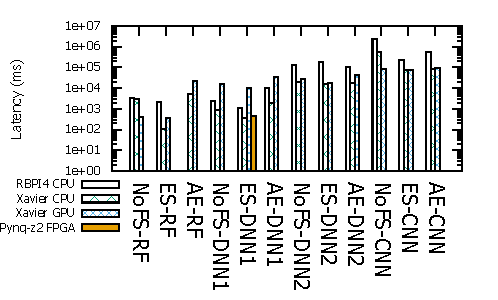
\includegraphics[width=0.9\columnwidth]{5_Chapitre5/figures/latency_bar.pdf}
    \caption{Latency characterization of IDS models.}
    \label{figure:herocache-performance}
\end{figure}

% TODO: Performances des supports de stockage : mesures (temps) en banc d'essai, facteur de ralentissement SotA pour les supports distants~\cite{wawrzoniakBoxerDataAnalytics2021a}

\subsection{Mesures de consommation d'énergie}

Nous avons exécuté des inférences sur les modèles d'IDS sur chaque élément de traitement et mesuré la consommation d'énergie de la plateforme à l'aide de l'analyseur de puissance N6705A DC. Les résultats sont présentés dans la figure~\ref{figure:herocache-energy}. Pour les mêmes raisons que mentionné ci-dessus, seul ES-DNN1 a été caractérisé sur FPGA. Nous observons que les plateformes CPU affichent une consommation d'énergie inférieure à celle du GPU dans la majorité des cas. Le seul cas où le GPU obtient de meilleurs résultats est lorsque la vitesse qu'il atteint par rapport aux CPU est élevée. C'est par exemple le cas pour NoFS-CNN, où le CPU RBPI4 est plus de 30 fois plus lent que le GPU. Même si la carte Pynq-Z2 présente la meilleure efficacité énergétique avec le modèle ES-DNN1, étant donné qu'elle est plus chère et présente une généricité limitée en matière de conception, nous supposons qu'elle est moins disponible que le RBPI4.

\begin{figure}
    \centering
    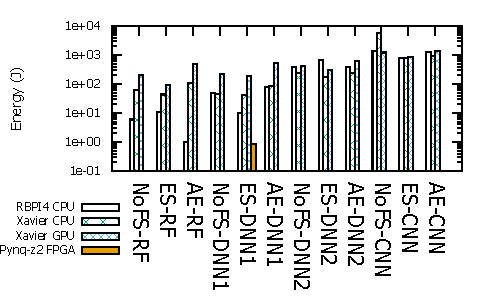
\includegraphics[width=0.9\columnwidth]{5_Chapitre5/figures/energy_bar.pdf}
    \caption{Energy characterization of IDS models.}
    \label{figure:herocache-energy}
\end{figure}

\section{Phase en ligne : orchestration avec HeROcache} \label{section:herocache-contribution}

\subsection{Présentation générale}

L'orchestrateur HeROcache est principalement composé de deux modules, un \textbf{autoscaler} et un \textbf{ordonnanceur} (voir figure~\ref{figure:herocache-serverless-platform}). L'autoscaler est chargé de l'allocation dynamique des ressources : il affecte les plateformes d'exécution aux répliques de fonctions. L'ordonnanceur s'occupe du placement des requêtes utilisateur sur les répliques.

HeROcache relève les trois défis susmentionnés en proposant des stratégies complémentaires de minimisation des coûts au niveau de l'autoscaler et de l'ordonnanceur. HeROcache minimise \textbf{les délais d'initialisation} en tenant compte des temps de latence induits par la récupération des images de fonctions au niveau de l'autoscaler. Une stratégie de \textit{prefetching} (ou \textit{prélecture}) est également mise en œuvre, qui consiste à essayer de mettre en cache des images de fonctions pertinentes en avance de phase. Les coûts de \textbf{communications inter-fonction} sont pris en compte principalement dans l'ordonnanceur, qui tend naturellement à consolider les fonctions d'une même application. L'autoscaler participe indirectement à cette consolidation par le \textit{prefetching}, en mettant en cache les fonctions suivantes du DAG de l'application sur le même nœud. Enfin, l'\textbf{hétérogénéité matérielle} est prise en compte car les différents facteurs de coût d'exécution extraits pendant la phase hors-ligne (voir section~\ref{section:herocache-workload}) sont exploités tout au long du processus d'autoscaling et d'ordonnancement. Les sections suivantes décrivent les stratégies de mise à l'échelle automatique et d'ordonnancement.

\subsection{Stratégie de minimisation des coûts d'allocation des ressources}

\begin{table}[!ht]
    \caption{Dictionnaire des notations}
    \begin{center}
    \scalebox{0.85}{
        \begin{tabularx}{\linewidth}{|c|Y|}
            \hline \textbf{Notation} & \textbf{Description} \\ \hline
            $x_a$ & Allocation des ressources pour une application $a$ \\ \hline
            $y_a$ & Invocation d'une application $a$ \\ \hline
            $z_i$ & Placement d'une tâche pour la fonction $i$ \\ \hline
            $f_{N, P}$ & Une fonction $f$ déployée pour exécution sur une plateforme $P$ disponible sur un nœud $N$ \\ \hline
            $f_{a}$ & Une fonction $f$ appartenant à une application $a$ \\ \hline
            $A$ & Nombre total d'applications disponibles pour déploiement sur la plateforme \\ \hline
            $F_{a}$ & Nombre total de fonctions appartenant à une application $a$ \\ \hline
            $RT_{{f}_{N, P}}$ & Temps de récupération de l'image de la fonction $f$ pour un déploiement sur une plateforme $P$ disponible sur un nœud $N$ \\ \hline
            $NB_{N}$ & Bande passante réseau disponible entre un nœud $N$ et l'infrastructure \\ \hline
            $SMT_{N}$ & Débit du support de stockage disponible sur un nœud $N$ \\ \hline
            $SML_{N}$ & Latence du support de stockage disponible sur un nœud $N$ \\ \hline
            $QP$ & Pénalité sur violation de qualité de service \\ \hline
            $QD$ & Facteur de ralentissement par niveau de qualité de service \\ \hline
            $WET$ & Pire temps d'exécution \\ \hline
            $TT$ & Temps total pour une tâche \\ \hline
            $CST$ & Temps de démarrage à froid \\ \hline
            $ST$ & Temps des opérations de stockage \\ \hline
            $ET$ & Temps d'exécution nominal d'une fonction \\ \hline
            $EC$ & Consommation d'énergie \\ \hline
            $IS$ & Taille de l'image d'une fonction \\ \hline
            $HP$ & Prix du matériel \\ \hline
            $TC$ & Consolidation des tâches \\ \hline
            $Q$ & File d'attente des requêtes dans une réplique \\ \hline
            $CP$ & Proportion de fonctions mises en cache sur un nœud pour une application donnée \\ \hline
            $SIS^{f}_{a}$, $SOS^{f}_{a}$ & Respectivement les tailles des données d'entrée et de sortie d'une fonction $f$ appartenant à une application $a$ \\ \hline
            $threshold_{f, h}$ & Seuil de concurrence pour une fonction $f$ sur un type de matériel $h$ \\ \hline
            $scaleCost^{{f}_{{i}_{N, P}}}_a$ & Coût de la création d'une nouvelle réplique pour une fonction $f_i$ d'une application $a$ sur une plateforme $P$ disponible sur un nœud $N$ \\ \hline
            $schedCost^{{f}_{{i}_{N, P}}}_a$ & Coût de l'ordonnancement d'une tâche pour une fonction $f_i$ d'une application $a$ sur une plateforme $P$ disponible sur un nœud $N$ \\ \hline
        \end{tabularx}
    }
    \label{table:herocache-notation}
    \end{center}
\end{table}

Nous formulons l'allocation des ressources comme un problème d'optimisation et nous le résolvons à l'aide d'un algorithme glouton simple. L'objectif de l'autoscaler est de minimiser la somme des coûts des allocations $scaleCost_{a}$ pour $y_a$ invocations de l'application $a$ (équation~\ref{eq:herocache-objective-allocation}), pour toutes les applications dans $A$, sous contrainte d'une infrastructure finie avec $x_a$ l'allocation de ressources pour l'application $a$ (équation~\ref{eq:herocache-constraint-allocation}).

\begin{equation}
    \forall A, \, \min \sum_{a = 0}^{A} y_a \cdot scaleCost_{a}
\label{eq:herocache-objective-allocation}
\end{equation}

\begin{equation}
    \text{s. t.} \, \sum_{a = 0}^{A} x_a \leq Total Resources
\label{eq:herocache-constraint-allocation}
\end{equation}

Le coût de l'allocation des ressources pour une application $a$ est la somme des coûts d'allocation pour les fonctions qui la composent (équation~\ref{eq:herocache-scale-cost-app}). Une réplique est allouée à une plateforme d'exécution.

\begin{equation}
    scaleCost_{a} = \, \sum_{i = 0}^{F_{a}} scaleCost^{{f}_{{i}_{N, P}}}_a
\label{eq:herocache-scale-cost-app}
\end{equation}

Chaque réplique de fonction a un coût d'allocation associé, car l'allocation dynamique des ressources matérielles introduit un temps de latence lors du traitement des requêtes utilisateur.

Nous avons conçu un modèle de coût (équation~\ref{eq:herocache-scale-cost-function}) pour l'allocation des ressources nécessaires au déploiement d'une fonction d'une application donnée. Il est composé de quatre éléments, dont nous devons minimiser la somme :

\begin{itemize}
    \item La \textit{proportion de cache} $CP$ traduit la dispersion des fonctions sur les différents nœuds edge. Plus le score est élevé, plus les fonctions sont dispersées sur les nœuds. La minimisation de ce terme permet de consolider les fonctions ;
    \item Le \textit{temps total} $TT$ représente le temps d'exécution total de la fonction. Il tient compte de la qualité de service de l'application, de l'hétérogénéité de la plateforme et du coût de déploiement (si l'image est mise en cache sur le nœud ou distante). Plus ce coût est élevé, plus la qualité de service est faible ;
    \item La \textit{consommation d'énergie} $EC$ traduit la consommation d'énergie du déploiement de la fonction. Plus $EC$ est élevé, plus le coût est important ;
    \item Le \textit{prix du matériel} $HP$ décrit le coût total de possession (\textit{TCO}, pour \textit{Total Cost of Ownership}) supporté par les fournisseurs de services en fonction du temps d'exécution. Il traduit le coût de déploiement sur une plateforme matérielle donnée. Plus $HP$ est élevé, plus le coût de la solution est important.
\end{itemize}

L'objectif global du modèle de coût est de déployer une fonction au coût le plus bas possible, c'est-à-dire avec une consolidation accrue, une réduction du \textit{makespan} (le temps total d'exécution), une réduction de la consommation d'énergie et une réduction du coût de possession. Nous détaillerons chaque partie de l'équation~\ref{eq:herocache-scale-cost-function} dans les paragraphes suivants. Chaque composante de l'équation est pondérée pour permettre un réglage souple ; les valeurs que nous avons choisies pour le déploiement de l'application d'IDS sont spécifiées dans la partie consacrée à l'évaluation (section~\ref{section:herocache-evaluation}).

\begin{equation}
\begin{split}
 \forall N, \forall P \in N, scaleCost^{{f}_{{i}_{N, P}}}_{a} = \,   &k_{CP} \cdot {CP}_{{a}_{N}}    \\
    + &k_{TT} \cdot {TT}_{{f}_{N, P}} \\
    + &k_{EC} \cdot {EC}_{{f}_{N, P}} \\
    + &k_{HP} \cdot {HP}_{{f}_{N, P}}
\end{split}
\label{eq:herocache-scale-cost-function}
\end{equation}

\textbf{Proportion de cache}. Comme nous l'avons vu précédemment, la mise en œuvre de la consolidation des tâches (donc des exécutions de fonctions) au sein des applications devrait permettre de minimiser les délais de communication qui pourraient s'accumuler au sein des chaînes de fonctions. HeROcache favorise le déploiement de répliques d'une fonction sur des nœuds où d'autres fonctions appartenant à la même application sont déjà déployées.

Pour ce faire, HeROcache surveille $CF_{a}^{{f}_{i_{N, P}}}$ le nombre d'images de fonctions ${f}_{i}$ de l'application $a$ déployée sur le nœud $N$ sur une plateforme d'exécution donnée $P$ (par exemple, GPU) disponibles en cache sur le stockage local du nœud. La proportion de fonctions mises en cache est calculée pour chaque application (équation~\ref{eq:herocache-cached-functions}), puis la moyenne est calculée sur toutes les applications s'exécutant sur un nœud donné. Enfin, on l'inverse pour obtenir une valeur élevée pour les applications peu consolidées (l'objectif étant de minimiser cette proportion), voir équation~\ref{eq:herocache-cache-proportion-app}.

\begin{equation}
    \forall a \in A, \, \forall f \in a, \, CF_{a}^{{f}_{i_{N, P}}} = \frac{\sum_{i = 0}^{Fa} isCached(f_{i}, N, P)}{F_{a}}
\label{eq:herocache-cached-functions}
\end{equation}

\begin{equation}
    \forall N, \forall P \in N, \, {CP}_{{a}_{N}} = \, \frac{A}{\sum_{i = 0}^{F_{a}} CF_{a}^{{f}_{i_{N, P}}}}
\label{eq:herocache-cache-proportion-app}
\end{equation}

En plus de la minimisation des coûts, afin de réduire les délais de déploiement, l'autoscaler essaie de mettre en cache les images des chaînes de fonctions en avance de phase, lors du déploiement d'une nouvelle réplique sur un nœud. Il inspecte les chaînes de fonctions et télécharge séquentiellement les images de fonctions manquantes du registre distant vers le stockage local du nœud, de manière asynchrone. Cette technique permet de réduire la latence des requêtes futures~\cite{leeSPESOptimizingPerformanceResource2024a}.

\textbf{Temps total}. La deuxième composante du coût de mise à l'échelle est le \textit{temps total}. La minimisation du temps total devrait empêcher les retards d'initialisation de faire boule de neige dans les chaînes de fonctions, évitant ainsi les violations des accords de niveau de service (SLA).

Grâce aux métadonnées collectées sur chaque fonction pendant la phase hors-ligne, l'autoscaler est en mesure de prédire le temps total ${TT}_{{f}_{N, P}}$ de la première requête qui sera ordonnancée sur une nouvelle réplique de fonction (équation~\ref{eq:herocache-total-time-function}).

\begin{equation}
    {TT}_{{f}_{N, P}} = \, {RT}_{{f}_{N, P}} + {WT}_{{f}_{N, P}} + {CST}_{{f}_{N, P}} + {ET}_{{f}_{N, P}}
\label{eq:herocache-total-time-function}
\end{equation}

\begin{itemize}
    \item ${RT}_{{f}_{N, P}}$ est la durée de récupération de l'image de la fonction. Si l'image de la fonction est déjà mise en cache sur le nœud de calcul, cette durée est nulle ; sinon, elle dépend de la taille de l'image $IS$ et est influencée par la bande passante $NB$ du lien réseau, car l'image sera lue à partir d'un registre d'images distant, et par le débit du support de stockage du nœud $SMT$ ainsi que sa latence $SML$, car l'image sera écrite et stockée localement en vue d'une utilisation ultérieure (équation~\ref{eq:herocache-retrieval-time}) ;

    \begin{equation}
        {RT}_{{f}_{N, P}} = \, \frac{IS_{{f}_{N, P}}}{\min (NB_{N}, SMT_{N})} + SML_{N}
        \label{eq:herocache-retrieval-time}
    \end{equation}

    \item ${WT}_{{f}_{N, P}}$ est le temps que la tâche passera à attendre dans la file d'attente de la plateforme. Au moment de la création de la réplique, ce temps sera égal à zéro car nous ne prévoyons que la latence encourue par la première requête sur la réplique ;
    \item ${CST}_{{f}_{N, P}}$ est le temps de démarrage à froid nécessaire pour initialiser l'instance de la fonction (\textit{i.e.} décompresser l'image, préparer le conteneur, initialiser les bibliothèques, etc.). Il est mesuré en fonction des métadonnées extraites lors de la phase hors-ligne ;
    \item ${ET}_{{f}_{N, P}}$ est la durée d'exécution de la fonction, y compris le temps de communication avec ses prédécesseurs et successeurs potentiels dans le DAG. Cette durée tient compte des métadonnées extraites pour la plateforme de déploiement (équation~\ref{eq:herocache-execution-time}).
\end{itemize}

\begin{equation}
    {ET}_{{f}_{N, P}} = \, {CT}_{{f}_{N, P}} + {ST}_{{f}_{N, P}}
\label{eq:herocache-execution-time}
\end{equation}

${CT}_{{f}_{N, P}}$ est le \textit{temps de calcul} de la fonction -- le temps attendu pour que la fonction termine son exécution une fois entièrement initialisée. Cette valeur dépend des performances et de la disponibilité de la plateforme d'exécution. ${ST}_{{f}_{N, P}}$ est le \textit{temps de stockage} de la fonction -- le temps attendu pour que la fonction récupère ses données d'entrée et stocke ses données de sortie. Cette valeur dépend des performances du lien réseau et des dispositifs de stockage, comme montré dans l'équation~\ref{eq:herocache-storage-time}.

\begin{equation}
    {ST}_{{f}_{N, P}} = \, \frac{SIS_{a}^{f_{i_{N, P}}} + SOS_{a}^{f_{i_{N, P}}}}{\min (NB_{N}, SMT_{N})} + SML_{N}
\label{eq:herocache-storage-time}
\end{equation}

\textbf{Consommation d'énergie et prix du matériel}. Enfin, la prise en compte de la consommation d'énergie et du prix du matériel devrait permettre de départager les candidats lorsque plusieurs allocations possibles semblent produire le même coût (en fournissant le même niveau de qualité de service).

${EC}_{{f}_{N, P}}$ et ${HP}_{{f}_{N, P}}$ correspondent respectivement (a) à la consommation d'énergie dynamique générée par cette allocation, obtenue grâce à la phase de caractérisation hors-ligne de la charge de travail et de la plateforme et (b) au prix catalogue suggéré par le fabricant (\textit{MSRP}, pour \textit{Manufacturer's Suggested Retail Price}) $Hardware Price_{P}$ du matériel mobilisé pour déployer la fonction sur ledit nœud et ladite plateforme, au regard du temps d'exécution de la fonction $ET_{{f}_{N, P}}$ (équation~\ref{eq:herocache-hardware-price}).

\begin{equation}
    {HP}_{{f}_{N, P}} = \frac{Hardware Price_{P}}{ET_{{f}_{N, P}}}
\label{eq:herocache-hardware-price}
\end{equation}

\subsection{Stratégie de minimisation des coûts d'ordonnancement et de placement des données}

Comme pour l'autoscaling, nous formulons un problème d'optimisation pour trouver la configuration d'ordonnancement optimale pour chaque requête utilisateur (puisque la qualité de service doit être garantie sur la base d'une requête utilisateur) et nous le résolvons à l'aide d'un simple algorithme glouton. L'objectif de l'ordonnanceur est de minimiser le coût du placement de $z_i$ tâches sur $R_i$ répliques de la fonction $i$ pour $y_a$ invocations de l'application $a$ (équation~\ref{eq:herocache-objective-scheduling}), sous contrainte d'un ensemble fini de répliques de fonction $R_{i}$ (équation~\ref{eq:herocache-constraint-scheduling}) précédemment déployée par l'autoscaler. Nous supposons que les applications sont toujours exécutées jusqu'au bout et que les nœuds ne tombent pas en panne ; il n'y a donc pas de coût associé aux migrations de tâches ou aux nouvelles tentatives.

\begin{equation}
    \min \sum_{a = 0}^{A} y_a \cdot schedCost_{a}
\label{eq:herocache-objective-scheduling}
\end{equation}

\begin{equation}
    \text{s. t.} \, \forall a \sum_{i = 0}^{F_a} z_i \leq \sum_{i = 0}^{F_a} R_{i}
\label{eq:herocache-constraint-scheduling}
\end{equation}

Comme la plateforme fonctionne à la granularité des fonctions, le coût d'ordonnancement d'une application $a$ est la somme du coût d'ordonnancement de sa chaîne de fonctions (équation~\ref{eq:herocache-scheduling-cost-app}).

\begin{equation}
    schedCost_{a} = \, \sum_{i = 0}^{A} schedCost^{{{f}_{i}}}_{a}
\label{eq:herocache-scheduling-cost-app}
\end{equation}

Chaque fonction ordonnancée dans la chaîne a un coût associé, calculé pour chaque placement possible sur une réplique existante. Nous avons conçu un modèle de coût (équation~\ref{eq:herocache-scheduling-cost-function}) pour le placement des tâches nécessaires au traitement d'une requête utilisateur pour une application.

\begin{equation}
    schedCost_{{f}_{{i}_{N, P}}} = \, k_{QP} \cdot QP_{{f}_{N, P}} + k_{EC} \cdot {EC}_{{f}_{N, P}} + k_{TC} \cdot TC_{{f}_{N, P}}
\label{eq:herocache-scheduling-cost-function}
\end{equation}

Ce modèle est composé de trois éléments, dont nous devons minimiser la somme :

\begin{itemize}
    \item La \textit{pénalité sur qualité de service} $QP$ est encourue par le fournisseur de services lorsqu'une requête utilisateur n'est pas traitée en temps voulu. Il s'agit d'une valeur booléenne qui détermine si, en raison d'un placement donné, l'application ne respectera pas son échéance ;
    \item La \textit{consommation d'énergie} $EC$ traduit la consommation d'énergie dynamique induite par l'exécution de la fonction. Plus $EC$ est élevée, plus le coût est important ;
    \item La \textit{consolidation des tâches} $TC$ décrit l'utilisation des ressources pour un placement donné. Plus $TC$ est faible, plus la file d'attente de la réplique est proche de son seuil de concurrence, ce qui maximise l'utilisation du matériel.
\end{itemize}

L'objectif global du modèle de coût est de placer les requêtes utilisateur dans les répliques de fonctions au coût le plus bas possible, c'est-à-dire en évitant les pénalités subies par le fournisseur de services en cas de dépassement de l'échéance de l'application au regard des besoins définis par l'utilisateur ; en utilisant les plateformes d'exécution les moins gourmandes en énergie possible ; et en appliquant un ratio d'utilisation élevé pour les ressources allouées à chaque fonction. Nous décrivons chaque partie de l'équation~\ref{eq:herocache-scale-cost-function} dans les paragraphes suivants. Chaque composante de l'équation est pondérée pour permettre un réglage flexible ; les valeurs que nous avons choisies pour le déploiement de l'application d'IDS sont spécifiées dans la partie consacrée à l'évaluation (section~\ref{section:herocache-evaluation}).

\textbf{Pénalité de qualité de service}. L'ordonnanceur sélectionne les tâches entrantes en fonction de leur \textbf{échéance la plus proche} (\textit{EDF}, pour \textit{Earliest Deadline First}), en s'appuyant sur les métadonnées de la fonction pour calculer un temps d'exécution dans le pire cas noté $WET$ (équation~\ref{eq:herocache-task-wet}). La requête utilisateur est associée à un niveau de qualité de service qui définit un facteur de ralentissement variable $QD$ appliqué au temps d'exécution de l'application. Ces deux éléments permettent d'identifier l'échéance pour la requête.

\begin{equation}
    \forall \, (N, P), \, WET_{f} = \, \max ET_{f_{N, P}}
\label{eq:herocache-task-wet}
\end{equation}

Nous pouvons prédire la pénalité de l'application en additionnant le temps total prévu pour ses tâches et en le comparant à l'échéance de l'application (somme des échéances des fonctions), comme montré dans l'équation~\ref{eq:herocache-scheduling-penalty}. Nous réutilisons l'équation~\ref{eq:herocache-total-time-function} pour calculer le temps total d'exécution d'une fonction ; cependant, ici, les composantes $RT$ et $CST$ seront nulles car la réplique a déjà été initialisée par l'autoscaler lors de l'allocation. $WT$ sera égal à la somme des temps d'exécution des tâches de priorité supérieure actuellement en file d'attente sur la réplique.

\begin{equation}
   QP_{a} = \, \sum_{i = 0}^{F_a} TT_{{f}_{{i}_{N, P}}} > \sum_{i = 0}^{F_a} WET_{f_{i}} \cdot QD_{a}
\label{eq:herocache-scheduling-penalty}
\end{equation}

En prenant en compte le temps de stockage dans le coût d'ordonnancement, nous cherchons à inciter l'ordonnanceur à placer les tâches aussi près que possible des données sur lesquelles elles opèrent. Pour éviter de saturer le stockage local des nœuds, la plateforme procède au nettoyage des données intermédiaires dès que l'application a terminé son exécution, \textit{i.e.} lorsque la dernière fonction de la chaîne retourne sa valeur.

\textbf{Consommation d'énergie}. ${EC}_{{f}_{N, P}}$ correspond à la consommation d'énergie dynamique générée par cette configuration d'ordonnancement. Elle est liée au temps d'exécution de la fonction. Les résultats des mesures hors-ligne sont utilisés pour déterminer ce terme.

\textbf{Consolidation des tâches}. Nous voulons que les files d'attente des répliques de fonctions atteignent leur seuil de concurrence : le pire cas est d'avoir une file d'attente vide, ce qui signifie que des ressources matérielles auraient été inutilement allouées. Nous voulons également empêcher les files d'attente de répliques de croître trop rapidement au-delà de ce seuil, car cela pourrait entraîner des violations de la qualité de service en raison de longs temps d'attente.

Nous commençons par établir le ratio d'\textit{utilisation de la plateforme} $PU$ de chaque réplique pour la fonction que nous essayons d'ordonnancer (équation~\ref{eq:herocache-platform-usage}) : plus la longueur de la file d'attente de la réplique $Q$ est proche de son seuil de concurrence ($threshold$ dans l'équation), plus le score est faible.

\begin{equation}
    PU_{f_{N, P}} = \frac{Q_{N, P}}{threshold_{f, P}}
\label{eq:herocache-platform-usage}
\end{equation}

Ensuite, nous calculons un score de consolidation des tâches $TC$ en appliquant une fonction exponentielle à $PU$ (équation~\ref{eq:herocache-task-consolidation}). Ainsi, $TC$ est le plus faible pour les placements dans les répliques inactives, et ce coût augmente fortement au fur et à mesure que les files d'attente se remplissent, ce qui conduit l'ordonnanceur à donner la priorité aux placements sur les répliques vides et à éviter les répliques où la file d'attente des requêtes est saturée.

\begin{equation}
    TC_{{f}_{N, P}} = \, exp(PU_{f_{N, P}})
\label{eq:herocache-task-consolidation}
\end{equation}

\section{Évaluation}
\label{section:herocache-evaluation}

Cette section présente notre méthodologie d'évaluation et les résultats obtenus dans un scénario de déploiement d'IDS sur des dispositifs edge. L'évaluation se fait en deux phases : nous comparons HeROcache à plusieurs stratégies de référence, puis nous évaluons l'impact de chacun de ses composants (autoscaler et ordonnanceur) pris séparément.

\begin{figure*}[t]
    \center
    \subfloat[Consolidation\label{figure:herocache-evaluation-full-unused-nodes}]{
        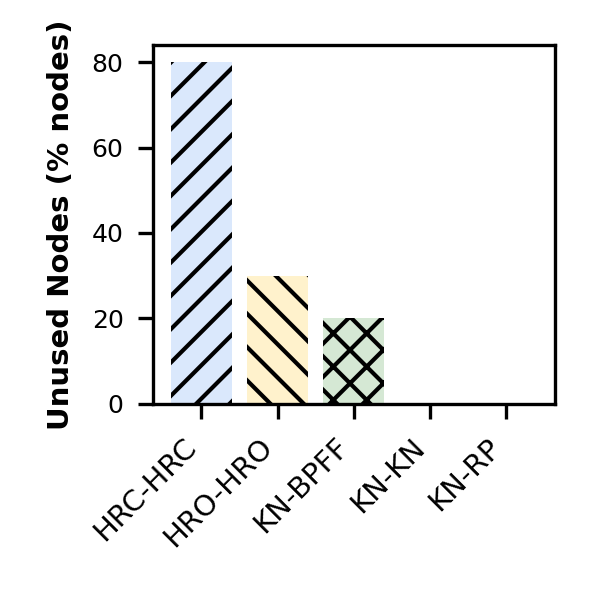
\includegraphics[width=0.155\linewidth]{5_Chapitre5/figures/eval/2-unused-nodes.png}
    }
    \subfloat[\gls{QoS}\label{figure:herocache-evaluation-full-penalty}]{
        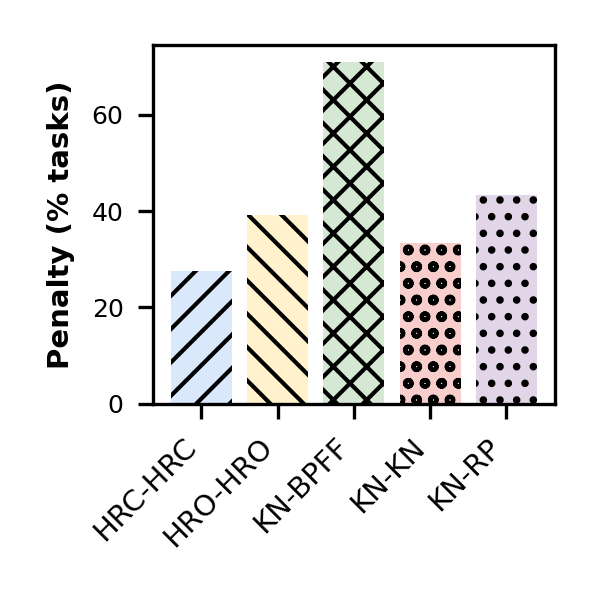
\includegraphics[width=0.155\linewidth]{5_Chapitre5/figures/eval/3-penalty-proportions.png}
    }
    \subfloat[Énergie\label{figure:herocache-evaluation-full-energy-consumption}]{
        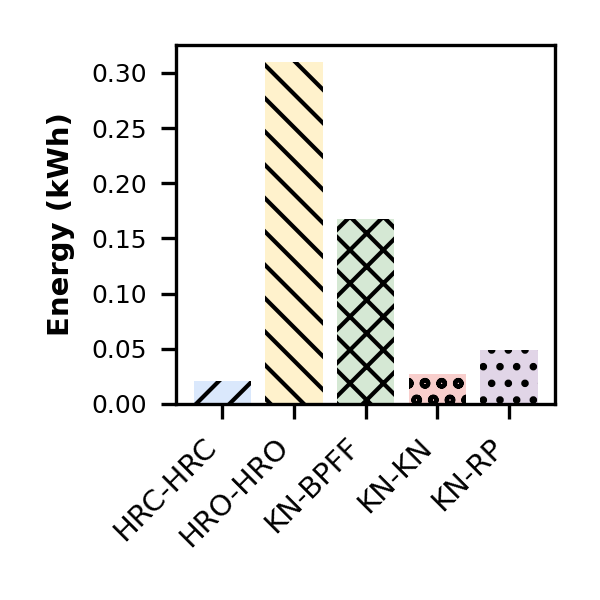
\includegraphics[width=0.155\linewidth]{5_Chapitre5/figures/eval/6-energy-consumption.png}
    }
    \subfloat[Consolidation\label{figure:herocache-evaluation-components-unused-nodes}]{
        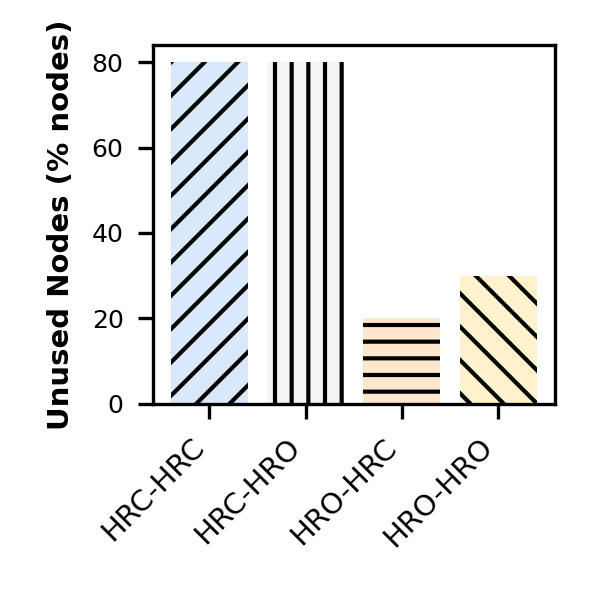
\includegraphics[width=0.155\linewidth]{5_Chapitre5/figures/eval-components/2-unused-nodes.png}
    }
    \subfloat[\gls{QoS}\label{figure:herocache-evaluation-components-penalty}]{
        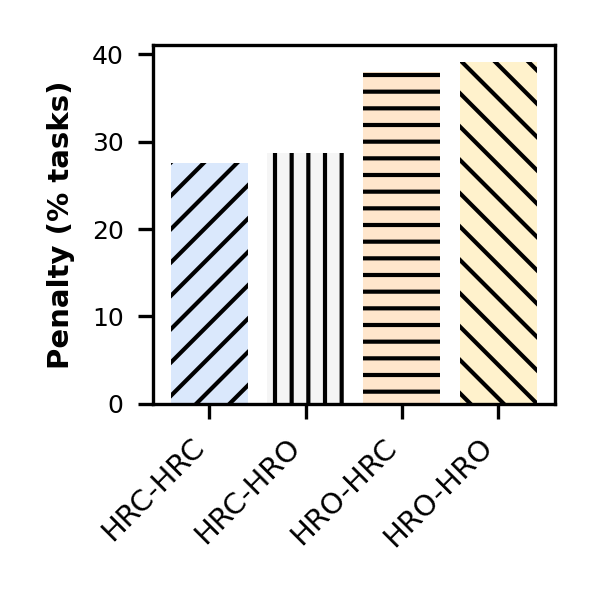
\includegraphics[width=0.155\linewidth]{5_Chapitre5/figures/eval-components/3-penalty-proportions.png}
    }
    \subfloat[Énergie\label{figure:herocache-evaluation-components-energy-consumption}]{
        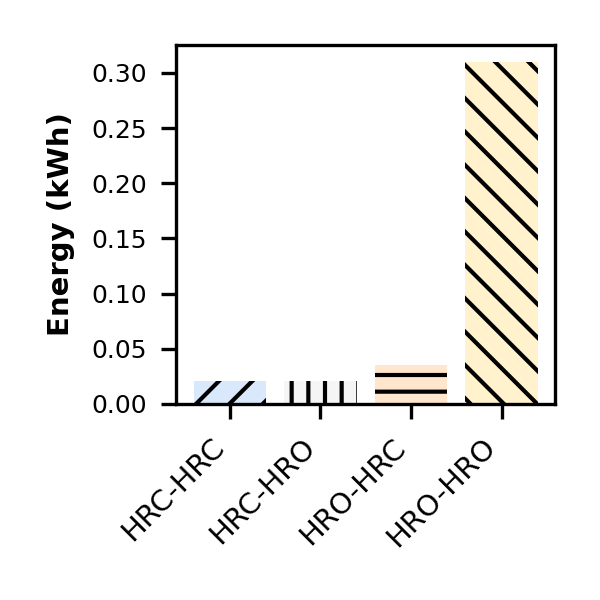
\includegraphics[width=0.155\linewidth]{5_Chapitre5/figures/eval-components/6-energy-consumption.png}
    }
    \caption{Évaluation -- Comparaison aux politiques de référence (a-c) et impact des composants individuels (d-f)}
    \label{figure:herocache-evaluation}
\end{figure*}

\subsection{Protocole expérimental}

\textbf{Métadonnées de caractérisation hors-ligne}. Pour évaluer notre contribution, nous avons effectué des mesures pour trois applications d'IDS (voir section~\ref{section:herocache-characterization-workloads}). Ces applications consistent en différentes combinaisons de fonctions de prétraitement et d'inférence, mises en œuvre sur du matériel hétérogène (voir section~\ref{section:herocache-characterization-platforms}). Ces métadonnées ont servi d'entrée à un simulateur à évènements discrets, HeROsim (voir chapitre~\ref{chapter:herosim}), utilisé pour estimer la pertinence de nos stratégies.

\textbf{Orchestration en ligne}. Nous avons généré des scénarios synthétiques en modélisant les requêtes utilisateur comme un processus de Poisson, suivant une distribution uniforme entre les invocations d'applications, comme couramment pratiqué dans l'état de l'art~\cite{9928755}. En modifiant le paramètre $\lambda$ du processus de Poisson, nous pouvons générer diverses traces avec différents taux de requêtes par seconde (\textit{RPS}). Nous avons envisagé un scénario avec 10 nœuds edge communiquant via un lien 4G (LTE). La bande passante pour la 4G LTE dépend de divers facteurs allant de la couverture de l'antenne à la qualité de service du fournisseur, en passant par la qualité du récepteur. Nous avons choisi d'utiliser une valeur représentative à 100 Mbps (12,5~MB/s). Les paquets \gls{TCP} à analyser ont une taille de 1,5~KB et sont envoyés par lots de 100 aux applications d'IDS. Cela donne un taux de 83~RPS dans notre scénario, pour 10 minutes de requêtes utilisateur.

Les pondérations pour les décisions de mise à l'échelle automatique (équation~\ref{eq:herocache-scale-cost-function}) ont été fixées à $k_{CP} = \frac{3}{8}$, $k_{TT} = \frac{3}{8}$, $k_{EC} = \frac{1}{8}$ et $k_{HP} = \frac{1}{8}$ dans le but de privilégier une latence faible à basse consommation d'énergie. Les pondérations pour les décisions d'ordonnancement (équation~\ref{eq:herocache-scheduling-cost-function}) ont été fixées à $k_{QP} = \frac{2}{3}$, $k_{EC} = \frac{0.5}{6}$ et $k_{TC} = \frac{1.5}{6}$ pour favoriser un faible nombre d'échéances manquées. Nous utilisons des valeurs inspirées de~\cite{herofake} afin d'être comparables.

Pour éviter une forme d'"emballement" (on parle de \textit{thrashing}) dans lequel les répliques sont créées et détruites en boucle lorsque la concurrence dans le système est très proche du seuil de concurrence, l'autoscaler applique un temps de maintien en vie (\textit{keep-alive delay}) faible qui empêche la destruction d'une réplique récemment allouée. Nous avons fixé ce temps de maintien en vie à 30 secondes, ce qui est la valeur par défaut dans Knative.

Dans nos expériences, nous nous autorisons à évaluer autoscalers et ordonnanceurs séparément afin de mieux comprendre leur comportement. Nous avons évalué différentes combinaisons pour montrer quelle composante de chaque politique est pertinente pour relever les différents défis de notre problème. Nous avons mis en œuvre trois autoscalers dans notre simulateur :

\begin{itemize}
    \item HeROcache (HRC) -- Notre politique de mise à l'échelle automatique repose sur la mise en cache d'images de fonctions sur les nœuds edge et tente d'anticiper la mise en cache des images de fonctions pour satisfaire les dépendances du DAG localement lors du déploiement d'applications ;
    \item HeROfake (HRO)~\cite{herofake} -- Applique une politique similaire à HRC, mais ne tient pas compte des coûts de stockage : l'ordonnanceur n'utilise pas le cache d'image local du nœud lors de l'instanciation des répliques de fonctions, et n'effectue pas non plus la recherche préalable des images de fonctions en fonction du DAG de leur application ;
    \item Knative (KN)~\cite{sureshENSUREEfficientScheduling2020} -- Nous avons modélisé le comportement de l'autoscaler de Knative du mieux que nous avons pu, en nous appuyant sur la documentation disponible au moment de cette étude~\cite{knative-autoscaling}. Il déploie les répliques de fonctions sur le nœud le plus disponible, \textit{i.e.} il effectue un équilibrage de charge.
\end{itemize}

En plus de ces autoscalers, nous avons utilisé quatre ordonnanceurs :

\begin{itemize}
    \item HeROcache (HRC) -- Notre politique d'ordonnancement sélectionne les requêtes utilisateur entrantes en fonction de leur échéance la plus proche afin de maximiser la qualité de service. Notre ordonnanceur tient compte de la latence de communication prévue et sélectionne une réplique en fonction des exigences de temps de réponse dictées par la requête ;
    \item HeROfake (HRO)~\cite{herofake} -- Applique une politique similaire à HRC, mais ne tient pas compte des coûts de stockage : l'ordonnanceur ne prédit pas la latence des communications dans le DAG de l'application ;
    \item Knative (KN)~\cite{knative} -- Knative considère les plateformes d'exécution comme homogènes et ne tient pas compte de la QoS requise par les utilisateurs. Les répliques sont triées en fonction du nombre de requêtes en attente ; la réplique ayant la file d'attente la plus courte est sélectionnée ;
    \item Bin-Packing First Fit (BPFF)-- Les tâches sont consolidées sur un nombre minimum de répliques. L'ordonnanceur place les requêtes sur une première réplique jusqu'à ce que celle-ci atteigne son seuil de concurrence. BPFF est susceptible d'être la politique d'ordonnancement mise en œuvre pour AWS Lambda~\cite{wangPeekingCurtainsServerlessb} ;
    \item Random Placement (RP) -- Les tâches sont ordonnancées sur une réplique sélectionnée de manière aléatoire.
\end{itemize}

Le nom de chaque scénario se compose de deux parties séparées par un tiret. La première partie correspond à la politique d'autoscaler ; la deuxième partie correspond à la politique d'ordonnancement (par exemple, HRC-KN signifie que nous avons utilisé l'autoscaler HeROcache avec l'ordonnanceur Knative).

Nous avons conçu une évaluation des performances en deux étapes : \\
(1) \textbf{Comparaison avec les politiques de référence} : nous comparons HeROcache complet (HRC-HRC) à : (1) Knative complet (KN-KN), (2) HeROfake complet (HRO-HRO), (3) l'autoscaler Knative avec l'ordonnanceur BPFF (KN-BPFF), (4) l'autoscaler Knative avec l'ordonnanceur RP (KN-RP). \\
(2) \textbf{Impact des composants individuels sur les performances globales} : nous discutons de l'impact respectif de l'autoscaler et de l'ordonnanceur dans différentes stratégies : (1) l'autoscaler HeROcache avec l'ordonnanceur HeROfake (HRC-HRO), et (2) l'autoscaler HeROfake avec l'ordonnanceur HeROcache (HRO-HRC), en les comparant aux versions complètes de HeROcache et HeROfake.

Nous évaluons HeROcache sur la base de trois mesures : (1) le nombre de nœuds inutilisés dans l'infrastructure, qui mesure le niveau de consolidation atteint ; (2) les pénalités sur qualité de service, qui expriment la capacité de notre stratégie à répondre aux exigences des utilisateurs ; (3) la consommation d'énergie, qui est un défi important à l'edge avec des ressources limitées.

\subsection{Analyse des résultats}

\subsubsection{Comparaison aux politiques de base}

\textbf{Consolidation des tâches}. La figure~\ref{figure:herocache-evaluation-full-unused-nodes} montre que notre combinaison d'autoscaler et d'ordonnanceur réalise la meilleure consolidation des tâches, en utilisant seulement 20\% de l'infrastructure edge pour l'exécution du scénario. Knative se comporte comme prévu, en répartissant la charge sur l'ensemble de l'infrastructure. On note que BPFF sous Knative produit des résultats légèrement différents : comme les files d'attente des tâches sont maximisées, l'autoscaler n'a pas besoin d'allouer autant de répliques. Dans ce scénario, si les nœuds edge inutilisés étaient mis hors tension au lieu de rester inactifs, notre stratégie permettrait au fournisseur de services d'économiser près de 100 Wh (soit 80\% de l'énergie statique et plus de 83\% de l'énergie totale) en mettant hors tension 80\% de l'infrastructure, tout en garantissant le temps de réponse des applications pour 72\% des requêtes utilisateur.

\textbf{Qualité de service}. La figure~\ref{figure:herocache-evaluation-full-penalty} illustre la pertinence de la prise en compte de l'hétérogénéité des ressources. En effet, notre politique parvient à maintenir les violations de la qualité de service à 27,5\% des requêtes tout en laissant 80\% de l'infrastructure inutilisée. Knative viole un peu plus de 30\% de la QoS des requêtes utilisateur tout en répartissant la charge sur tous les nœuds edge disponibles, ce qui est contre-intuitif. Cela s'explique par les dépendances entre les tâches que Knative ne prend pas en compte. En conséquence, les tâches ont tendance à communiquer \textit{via} le réseau, sur un support de stockage lent. Ainsi, bien que les tâches dans Knative passent en moyenne moins de temps en file d'attente, elles présentent toujours une latence plus élevée que dans HeROcache. Lors de l'utilisation de la politique BPFF, les violations atteignent presque 70\% : dans cette situation, les files d'attente des répliques sont trop longues pour que les requêtes puissent être traitées dans les délais impartis. À titre de comparaison, Knative utilisant l'ordonnanceur RP maintient les violations de la QoS autour de 50\%. HeROfake génère 39\% de violations de la qualité de service.

Notre politique maintient la proportion de démarrages à froid en dessous de 0,011\% des requêtes utilisateur, alors que Knative souffre de 4 fois plus de démarrages à froid. Dans HeROcache, le cache d'images local au nœud est utilisé dans 33\% des initialisations de fonctions, ce qui réduit les délais d'initialisation de 17,6\%.
Avec HeROcache, 30\% des tâches parviennent à communiquer par le biais du stockage local au niveau du nœud, ce qui accélère l'exécution de l'application en réduisant la latence des communications de 88,4\%.

\textbf{Consommation d'énergie}. La figure~\ref{figure:herocache-evaluation-full-energy-consumption} montre que HeROcache parvient à réduire la consommation d'énergie dynamique d'un tiers : avec un \textit{makespan} de 1505 secondes pour le scénario, l'infrastructure consomme 0,0088 kWh, contre 0,0266 kWh pour 2193 secondes de temps d'exécution sous Knative. Non seulement la stratégie de consolidation de HeROcache permettrait d'appliquer des politiques de mise hors tension susceptibles de réduire considérablement les besoins en énergie statique pour l'exécution d'applications d'IDS à l'edge, mais en sélectionnant des plateformes d'exécution adéquates, elle réduit également la consommation globale de l'infrastructure. HeROfake consomme le plus d'énergie (0,31 kWh) en raison d'un temps d'exécution beaucoup plus long pour le scénario.

\subsubsection{Impact des composants individuels}

\textbf{Consolidation des tâches}. La figure~\ref{figure:herocache-evaluation-components-unused-nodes} montre que les stratégies qui ne tiennent pas compte des coûts de stockage ne parviennent pas à consolider les tâches aussi bien que HeROcache : HRO-HRC et HRO-HRO utilisent respectivement 80\% et 70\% de l'infrastructure. Nous expliquons ces résultats de la manière suivante : les dépendances n'étant pas satisfaites à temps, la charge mesurée pour les différentes fonctions déployées continue d'augmenter, ce qui conduit l'autoscaler à incrémenter le nombre de répliques, enrôlant ainsi plus de nœuds pour la durée du scénario.

\textbf{Qualité de service}. La figure~\ref{figure:herocache-evaluation-components-penalty} illustre la conséquence du point précédent : les pénalités sur qualité de service sont plus élevées avec un autoscaler qui ne tient pas compte des délais introduits par la récupération des images de fonctions et les communications entre les fonctions. Bien que HRO-HRC soit conscient de l'hétérogénéité du matériel et des requêtes, il termine tout de même avec 37,9\% des applications qui ne respectent pas leur échéance.

\textbf{Consommation d'énergie}. La figure~\ref{figure:herocache-evaluation-components-energy-consumption} montre que, bien que HRO-HRC alloue 70\% de l'infrastructure, il parvient à maintenir une consommation d'énergie presque aussi faible que HRC-HRC. Cela s'explique par le fait qu'il a choisi les nœuds les moins gourmands en énergie, au prix de pénalités qu'il ne pouvait pas prévoir puisqu'il n'est pas conscient des enjeux liés au stockage.

\textbf{Note sur la complexité.} HeROcache utilise une technique d'optimisation gloutonne comparable à HeROfake. Dans HeROcache, la complexité est bornée par le nombre d'applications $A$, leur taille $f_{a}$ et la taille de l'infrastructure $N$ (équation~\ref{eq:herocache-complexity-autoscaler}) : dans le pire des cas, où toutes les ressources sont disponibles, l'autoscaler parcourt l'ensemble de l'infrastructure $N$ pour évaluer chaque nœud en vue de la création de répliques.

\begin{equation}
    \mathcal{O}_{autoscaling}(A \cdot f_{a} \cdot N)
\label{eq:herocache-complexity-autoscaler}
\end{equation}

Comme l'ordonnanceur travaille avec les répliques de fonctions déjà créées $R_{f}$, sa complexité est moindre (équation~\ref{eq:herocache-complexity-scheduler}).

\begin{equation}
    \mathcal{O}_{scheduling}(A \cdot f_{a} \cdot R_{f})
\label{eq:herocache-complexity-scheduler}
\end{equation}

Comme notre étude de cas actuelle implique un sous-ensemble limité de fonctions d'IDS avec un nombre raisonnable de nœuds edge, la complexité de l'algorithme n'a pas posé de problème. Toutefois, ce coût devrait être pris en compte pour des déploiements plus larges, pour différentes études de cas. Ce coût n'a pas été mesuré en simulation. Toutefois, comme l'autoscaler fonctionne de manière périodique, sa fréquence pourrait être ajustée en fonction des besoins et des contraintes du fournisseur de services. L'ordonnanceur est appelé au moment des requêtes utilisateur et pourrait être réparti sur les nœuds si la charge est trop lourde à gérer, au prix d'une vue d'ensemble instantanée de l'infrastructure.

\section{Travaux connexes}
\label{section:herocache-sota}

Des travaux antérieurs se sont concentrés sur les plateformes de mise à l'échelle automatique pour le déploiement de tâches de courte durée, comprises dans des applications présentant des modèles de charge imprévisibles (voir tableau~\ref{table:herocache-sota}).

Parmi ces travaux, \cite{smithFaDOFaaSFunctions2022} propose un orchestrateur conscient des dépendances de données, mais ne tenant pas compte de l'effet boule de neige des retards dans les chaînes de fonctions. \cite{zhangFIRSTExploitingMultiDimensional2023} ne prend pas en charge l'ordonnancement de ces chaînes de fonctions.
Toutes ces contributions considèrent une infrastructure homogène~\cite{bhasiCypressInputSizesensitive2022, zijunFassflowEfficient2022, smithFaDOFaaSFunctions2022, zhangFIRSTExploitingMultiDimensional2023, abdiPaletteLoadBalancing2023}. Cela n'est pas représentatif de notre cas d'utilisation, dans lequel les dispositifs edge sont très hétérogènes. HeROfake~\cite{herofake} exploite l'hétérogénéité matérielle dans sa politique d'orchestration, mais n'intègre pas les dépendances inter-fonctions ni la mise en cache des images dans son modèle de coût. Elle a été choisie à des fins d'évaluation, pour souligner la nécessité de prendre en compte ces coûts.
Certaines de ces contributions optimisent la consommation d'énergie au niveau de l'autoscaler \cite{bhasiCypressInputSizesensitive2022, zhangFIRSTExploitingMultiDimensional2023}. Toutefois, elles se concentrent sur la partie dynamique de la consommation d'énergie : elles ne tiennent pas compte de l'impact possible de la consolidation sur la consommation d'énergie statique. Nous soutenons que les fournisseurs de services devraient chercher à consolider les tâches afin de mettre hors tension le plus grand nombre de nœuds possible, ce qui réduirait considérablement les besoins énergétiques globaux de leurs infrastructures.
Dans \cite{fuerstIluvatarFastControl2023}, les auteurs ont étudié les différents coûts induits par la complexité de l'orchestration serverless. Cet élément n'a pas été pris en compte dans notre étude, car nous visons une infrastructure edge de taille limitée pour le déploiement d'applications d'IDS bien identifiées.

\section{Conclusion et perspectives}
\label{section:herocache-conclusion}

Dans ce chapitre, nous avons présenté une politique d'allocation et d'ordonnancement pour le serverless à l'edge. Cette politique cherche à optimiser le déploiement d'applications sensibles au temps pour la qualité de service sur des dispositifs à énergie limitée. En tirant parti de la caractérisation de la charge de travail, de l'hétérogénéité du matériel et des dispositifs de stockage locaux sur les nœuds edge, HeROcache consolide les applications et parvient à réduire les délais d'initialisation moyens de 17,6\% et les délais de communication de 88,4\%. Cela permet de réduire la consommation d'énergie statique de la plateforme de 80\% tout en maintenant moins de 28\% de violations de la qualité de service. Nous prévoyons de généraliser l'approche HeROcache pour des études de cas incluant plusieurs types d'applications sur des infrastructures plus importantes, à l'edge ou dans le cloud. Dans ce cas, des stratégies d'apprentissage automatique ou des métaheuristiques pourraient être utilisées à des fins de passage à l'échelle.
